\documentclass[11pt, twoside, openright, a4paper, chapterprefix]{scrbook}
\usepackage[inner=2.5cm, outer=2.5cm, top=4cm, bottom=4cm]{geometry}

%%% PACKAGES %%%%%%%%%%%%%%%%%%%%%%%%%%%%%%%%%%%%%%%%%%%%%%%%%%%%%%%%%%%%%%%%%%
%%%%%%%%%%%%%%%%%%%%%%%%%%%%%%%%%%%%%%%%%%%%%%%%%%%%%%%%%%%%%%%%%%%%%%%%%%%%%%%
%%
%%          $Id: packages.tex 385 2013-02-12 21:53:10Z holz $
%%    author(s): RoboCupAtWork Technical Committee(s)
%%  description: List of packages for the RoboCupAtWork rulebook
%%
%%%%%%%%%%%%%%%%%%%%%%%%%%%%%%%%%%%%%%%%%%%%%%%%%%%%%%%%%%%%%%%%%%%%%%%%%%%%%%%
\usepackage{soul}

\usepackage[english]{babel}
\usepackage{amsmath,amssymb,amsfonts}
\usepackage[nice]{nicefrac}
\usepackage{siunitx}
\usepackage{graphicx}
\usepackage{multicol}
\usepackage{verbatim}
\usepackage{fancyhdr}
% \usepackage{svn-multi}
\usepackage{color}
\usepackage{xcolor,colortbl}
\usepackage{epsfig}
\usepackage{makeidx}
\usepackage{lscape}
\usepackage{pdflscape}
\usepackage{picinpar}
% \usepackage{./styles/bar}
\usepackage{./styles/tweaklist}
\usepackage{subfig}
\usepackage{enumerate,paralist}
\usepackage{multirow}
\usepackage{pgffor}
\usepackage{array}
\usepackage{etoolbox}
\usepackage{hyperref}
\usepackage{tabularx}
\usepackage{xspace}
\usepackage[colorinlistoftodos]{todonotes}

%\usepackage[utf8x]{inputenc}
%\usepackage{times}
%\usepackage{helvet}
%\usepackage{courier}

\usepackage{url}
\usepackage{caption}
%\usepackage{subcaption}
\usepackage{epstopdf}
%\usepackage{subcaption}
\usepackage{float}
\usepackage{wrapfig}
%\usepackage{titlesec}
\usepackage{xfrac}

\usepackage[normalem]{ulem}  % used for \revadd, \revdel, etc.
\usepackage{xspace}  % used for adding spaces to macros, e.g. \RC, \RCAW, etc.
\usepackage[export]{adjustbox}  % used for valign option on images

\usepackage{pgfplots}
\usepgfplotslibrary{polar}

% Local Variables:
% TeX-master: "../Rulebook"
% End:

\usepackage[titletoc]{appendix}
\usepackage{enumitem}
\usepackage{mathtools}
\usepackage{gensymb}
\setlist{noitemsep}
\usepackage{hhline}
\usepackage{rotating}
\usepackage{tikz}
\usetikzlibrary{arrows}
\usetikzlibrary{calc}
\usetikzlibrary{decorations.pathreplacing}

%%% SubfigureSetup %%%%%%%%%%%%%%%%%%%%%%%%%%%%%%%%%%%%%%%%%%%%%%%%%%%%%%%%%%%%
%\renewcommand{\subfigtopskip}{5pt}        % default is 10pt
%\renewcommand{\subfigbottomskip}{5pt}     % default is 10pt
%\renewcommand{\subfigcapskip}{3pt}        % default is 10pt
%\renewcommand{\subfigcapmargin}{7pt}      % default is 10pt

%%% TweakList-Setup %%%%%%%%%%%%%%%%%%%%%%%%%%%%%%%%%%%%%%%%%%%%%%%%%%%%%%%%%%%
\renewcommand{\itemhook}{%                 % modify itemize-spacing
  \setlength{\topsep}{2pt}%
  \setlength{\partopsep}{1pt}%
  \setlength{\itemsep}{-1pt}%
}
\renewcommand{\enumhook}{%                 % modify enumerate-spacing
  \setlength{\topsep}{2pt}%
  \setlength{\partopsep}{1pt}%
  \setlength{\itemsep}{-1pt}%
}
\renewcommand{\descripthook}{%             % modify description-spacing
  \setlength{\topsep}{2pt}%
  \setlength{\partopsep}{1pt}%
  \setlength{\itemsep}{-1pt}%
}

\setkomafont{title}{\normalfont}
\setkomafont{sectioning}{\normalfont\bfseries}
\addtokomafont{caption}{\small}
\setkomafont{captionlabel}{\small\bfseries}
\setkomafont{descriptionlabel}{\normalfont\bfseries}
\renewcommand*{\chapterformat}{\LARGE{Chapter \thechapter}}


\setlength{\parskip}{10pt plus 1pt minus 1pt}
\setlength{\parindent}{0pt}

%%% MACROS %%%%%%%%%%%%%%%%%%%%%%%%%%%%%%%%%%%%%%%%%%%%%%%%%%%%%%%%%%%%%%%%%%%%
\newcommand{\YEAR}{2017\xspace}
\newcommand{\STATE}{First Draft}

\graphicspath{{\YEAR/}{./images/}}
%%%%%%%%%%%%%%%%%%%%%%%%%%%%%%%%%%%%%%%%%%%%%%%%%%%%%%%%%%%%%%%%%%%%%%%%%%%%%%%
%%
%%          $Id: macros.tex 399 2013-02-14 20:24:02Z holz $
%%    author(s): RoboCupAtHome Technical Committee(s)
%%  description: Macros for the RoboCupAtWork rulebook
%%
%%%%%%%%%%%%%%%%%%%%%%%%%%%%%%%%%%%%%%%%%%%%%%%%%%%%%%%%%%%%%%%%%%%%%%%%%%%%%%%

\input{./setup/macros_score_sheets.tex}
\input{./setup/macros_open_demonstrations.tex}

\newcommand{\rulebookVersion}{\STATE\ version for RoboCup \YEAR}

\def\RC{RoboCup\xspace}
\def\RCAW{RoboCup@Work\xspace}

\renewcommand{\labelenumi}{\arabic{enumi}.}
\renewcommand{\labelenumii}{\labelenumi\arabic{enumii}.}
\renewcommand{\labelenumiii}{\labelenumii.\arabic{enumiii}.}


%% %%%%%%%%%%%%%%%%%%%%%%%%%%%%%%%%%%%%%%%%%%%%%%%%%%%%%%%%% %%
%%                    Developement-Tools                     %%
%% %%%%%%%%%%%%%%%%%%%%%%%%%%%%%%%%%%%%%%%%%%%%%%%%%%%%%%%%% %%

%% %%%%%%%%%%%%%%%%%%%%%%%%%%%%%%%%%%%%%%%
\newcommand{\tbc}[1]{\textbf{\it\color{red}{t.b.c. ...}#1\color{black}}}
\newcommand{\chk}[1]{\textbf{\color{red}#1\color{black}}}

\newcommand{\revadd}[1]{\textcolor{blue}{#1}}
\newcommand{\revdel}[1]{\textcolor{red}{\sout{#1}}}
\newcommand{\revcha}[2]{\revdel{#1}\revadd{#2}}

\newcommand{\reworkon}{\marginpar{\raggedright\color{red}{$\downarrow$rework}\color{black}}}
\newcommand{\reworkoff}{\marginpar{\raggedright\color{red}{$\uparrow$rework}\color{black}}}

%% %%%%%%%%%%%%%%%%%%%%%%%%%%%%%%%%%%%%%%%
%%  site notes/margin notes
\def\note#1{\marginpar{\raggedright\tiny\color{blue}#1}}
\def\mpar#1{\marginpar{\raggedright\tiny#1}}
\def\rand#1{\marginpar{\raggedright\tiny#1}}
\setlength{\marginparwidth}{2cm}

\newcommand{\refsec}[1]{Section~\ref{#1}}
\newcommand{\reftab}[1]{Table~\ref{#1}}
\newcommand{\reffig}[1]{Figure~\ref{#1}}

%% %%%%%%%%%%%%%%%%%%%%%%%%%%%%%%%%%%%%%%%
%% side-annotation-macros for easy lookup
% \newcommand{\awardmark}{\marginpar{\centering\includegraphics[width=.34cm]{images/icon_award.pdf}}}
% \newcommand{\refmark}{\marginpar{\centering\includegraphics[width=.5cm]{images/icon_whistle.pdf}}}
% \newcommand{\referee}[1]{\emph{#1}\marginpar{\centering\includegraphics[width=.5cm]{images/icon_whistle.pdf}}}
% \newcommand{\scoremark}{\marginpar{\centering\includegraphics[width=.34cm]{images/icon_score.pdf}}}
\newcommand{\awardmark}{}
\newcommand{\refmark}{}
\newcommand{\referee}[1]{}
\newcommand{\scoremark}{}
%\newcommand{\scoring}[1]{\emph{#1}\marginpar{\centering\includegraphics[width=.34cm]{images/icon_score.pdf}}}
\newcommand{\scoring}[1]{\emph{#1}}
\newcommand{\timark}{\marginpar{\centering\includegraphics[width=.34cm]{icon_clock.pdf}}}

%\newcommand{\timing}[1]{\emph{#1}\marginpar{\centering\includegraphics[width=.34cm]{images/icon_clock.pdf}}}
\newcommand{\timing}[1]{\emph{#1}}

\def\svnRevision{Unknown} %
\def\svnChangeData{Unknown} %
\def\revnumtmpfile{.temp_rulebook_version}
\def\revdattmpfile{.temp_rulebook_date}
\immediate\write18{git rev-list HEAD | wc -l > \revnumtmpfile}
%\immediate\write18{svnversion . > \revnumtmpfile}
\IfFileExists{\revnumtmpfile}{\def\svnRevision{\input{\revnumtmpfile}\unskip}}{}
\immediate\write18{git log -1 --date=short  | grep 'Date:' | awk '{print $2}'> \revdattmpfile}
%\immediate\write18{svn info | grep 'Last Changed Date:' | awk '{print $4}'> \revdattmpfile}
\IfFileExists{\revdattmpfile}{\def\svnChangeData{\input{\revdattmpfile}\unskip}}{}
% \IfFileExists{\revnumtmpfile}{\immediate\write18{rm -f \revnumtmpfile}}{}
% \IfFileExists{\revdattmpfile}{\immediate\write18{rm -f \revdattmpfile}}{}
\newcommand{\VERSION}{Revision \svnChangeData\_\svnRevision}


% Local Variables:
% TeX-master: "../Rulebook"
% End:

\input{./setup/abbrevix.tex}



\makeindex                                % generate index
\makeabbex                                % generate abbreviations

%%% DOCUMENTINFO %%%%%%%%%%%%%%%%%%%%%%%%%%%%%%%%%%%%%%%%%%%%%%%%%%%%%%%%%%%%%%
\hypersetup{
  pdftitle     = {RoboCup@Work Rulebook},
  pdfsubject   = {RoboCup@Work Rulebook},
  pdfauthor    = {RoboCup@Work Technical Committee},
  pdfkeywords  = {RoboCup, @Work, Rules, Competition},
  colorlinks   = true,
  anchorcolor  = blue,
  linkcolor    = blue,
  urlcolor     = blue,
}

%%% HEADINGS & PAGE STYLE %%%%%%%%%%%%%%%%%%%%%%%%%%%%%%%%%%%%%%%%%%%%%%%%%%%%%
\newcommand{\footline}{RoboCup@Work Rulebook / \rulebookVersion}
\pagestyle{fancy}
\renewcommand{\chaptermark}[1]{\markboth{\chaptername\ \thechapter. \ #1}{}}
\renewcommand{\sectionmark}[1]{\markright{\thesection \ #1}{}\renewcommand{\currentTest}{#1}}
\fancyhf{}
\fancyhead[LE,RO]{\thepage}
\fancyhead[RE]{\sffamily\rightmark}
\fancyhead[LO]{\sffamily\leftmark}
\fancyfoot[C]{\scriptsize \sffamily \footline{}}
\fancypagestyle{plain}{
        \fancyhf{}
        \fancyhead[LE,RO]{\thepage}
        \fancyhead[RE]{\sffamily\rightmark}
        \fancyhead[LO]{\sffamily\leftmark}
        \fancyfoot[C]{\scriptsize \sffamily \footline{}}
		\renewcommand{\headrulewidth}{0.5 pt}
}
\fancypagestyle{empty}{
        \fancyhf{}
        \fancyhead{}
        \fancyfoot[C]{\scriptsize \sffamily \footline{}}
		\renewcommand{\headrulewidth}{0 pt}
}

\newcommand{\quotes}[1]{``#1''}
\newcommand{\textbi}[1]{\textbf{\textit{#1}}}
%\newcommand{\sectionbreak}{\clearpage}
%\newcommand{\subsectionbreak}{\clearpage}


%%%%%%%%%%%%%%%%%%%\renewcommand{%%%%%%%%%%%%%%%%%%%%%%%%%%%%%%%%%%%%%%%%%%%%%%%%%%%%%%%%%%%%
%%%%%%%%%%%%%%%%%%%%%%%%%%%%%%%%%%%%%%%%%%%%%%%%%%%%%%%%%%%%%%%%%%%%%%%%%%%%%%%
%%%%%%%%%%%%%%%%%%%%%%%%%%%%%%%%%%%%%%%%%%%%%%%%%%%%%%%%%%%%%%%%%%%%%%%%%%%%%%%

\begin{document}

% !TEX root = ../Rulebook.tex

\begin{titlepage}
  \begin{center}
    {

      \includegraphics[width=\textwidth]{images/logo_RoboCupAtWork.pdf}\\[1.23ex]
    }
    \vspace{2.7 cm}
    \hrulefill\par
    {%
      \vspace*{.27cm}
      \Huge{\RCAW}\\[1.23ex]
      \Large Rulebook \\[2ex]
    }

    \hrulefill\par

\szug{Check name list}

    \vfill
    Asadollah Norouzi\\
  	Sebastian Zug\\
    Jon Martin \\
    Deebul Nair \\
    Christoph Steup \\
    Marco Masannek\\
    Maximilian Hachen
    \vfill
    ~~ Version: \YEAR ~~ \\
    ~~  \today ~~ \\
    %\vfill
  \end{center}

\newpage

\section*{Acknowledgments}

We would like to thank to previous @Work members that supported the league and
advanced the rulebook over years:

Jan Carstensen \\
Frederik Hegger\\
Nico Hochgeschwender \\
Daniel Kaczor \\
Robin Kammel \\
Alexander Moriaty \\
Walter Nowak \\
Benjamin Schnieders\\
Armin Shahsavari \\

In July 2019 our league lost one of the initiators and founding members. Prof. Dr. Gerhard
Kraetzschmar has been very active in many functions within the RoboCup-Community
for decades. We are grateful for his efforts, advises and motivation and will respect his memory.

\section*{How to cite this rulebook}

If you refer to the rulebook in particular, please cite:

\szug{Check authors name list according to commits.}

\begin{verbatim}
@misc{rulebook_2020,
  author = {Asadollah Norouzi, Sebastian Zug, Jon Martin, Deebul Nair,
            Christoph Steup, Marco Masannek},
  title  = {RoboCup@Work 2020 - Rulebook},
  year   =  2020,
  howpublished = {\url{https://atwork.robocup.org/rules/}},
}
\end{verbatim}

\end{titlepage}



\pagestyle{empty}
\tableofcontents
\clearpage

\pagestyle{plain}

\chapter{Introduction}

\section{RoboCup@Work in a Nutshell}\label{sec:at_work_nushell}
RoboCup@Work is a new competition in RoboCup that targets the use of robots in work-related scenarios. RoboCup@Work utilizes proven ideas and concepts from RoboCup competitions to tackle open research challenges in industrial and service robotics. With the introduction of this new event, RoboCup opens up to communities researching both classical and innovative robotics scenarios with very high relevance for the robotics industry. 
\par
Examples for the work-related scenarios targeted by RoboCup@Work include 

\begin{itemize}
	\item loading and/or unloading of containers with/of objects with the same 	or different size,
	\item pickup or delivery of parts from/to structured storages and/or 				unstructured heaps,
	\item operation of machines, including pressing buttons, opening/closing 			doors and drawers, and similar operations with underspecified or unknown 			kinematics,
	\item flexible planning and dynamic scheduling of production processes 			involving multiple agents (humans, robots, and machines),
	\item cooperative assembly of non-trivial objects, with other robots 				and/or humans,
	\item cooperative collection of objects over spatially widely  distributed 	areas, and
	\item cooperative transportation of objects (robots with robots, robots 			with humans).
\end{itemize}

The RoboCup@Work scenarios target difficult, mostly unsolved problems in robotics, artificial intelligence, and advanced computer science, in particular in perception, path planning and motion planning, mobile manipulation, planning and scheduling, learning and adaptivity, and probabilistic modeling, to name just a few. Furthermore, RoboCup@Work scenarios may also address problems for which solutions require the use and integration of semantic web technology, RFID technology, or advanced computational geometry.
\par

Solutions to the problems posed by RoboCup@Work require sophisticated and innovative approaches and methods and their effective integration. The scenarios are defined such that the problems are sufficiently general and independent of particular industrial applications, but also sufficiently close to real application problems that the solutions can be adapted to particular application problems with reasonable effort.  
\par

A RoboCup@Work competition has only recently become a feasible idea for several reasons: The arrival of new, small, and flexible robot systems for mobile manipulation allow more university-based research labs to perform research in the above-mentioned areas. Advances and a revived interest in the use of simulation technology in robotics enable research groups to perform serious research without having a full set of costly robotics and automation equipment available. 
\par

The robotics and automation industry is recently shifting its attention towards robotics scenarios involving the integration of mobility and manipulation, larger-scale integration of service robotics and industrial robotics, cohabitation of robots and humans, and cooperation of multiple robots and/or humans. Last but not least, there is a huge interest by funding agencies and professional societies in well-designed and professionally performed benchmarks for industry-relevant robotics tasks. RoboCup@Work is designed as an instrument to serve all these needs. 


\section{Organization of the League}\label{sec:organisation_of_the_league}

\subsection{League Committees}
The following list of committees is implemented for RoboCup@Work.

\subsubsection{Executive Committee}

Executive Committee (EC) members are responsible for the long term goals of the league and thus have also contact to other leagues as well as to the RoboCup federation. The Executive Committee presents the league and its achievements to the RoboCup federation every year and gets feedback to organize the league. All committee members are also members of the Technical Committee. Executive Committee members are elected by the Board of Trustees and appointed by the President of the RoboCup Federation, they serve 3-year terms.

\begin{itemize}
	\item Walter Nowak, Locomotec GmbH
	\item Nico Hochgeschwender, Bonn-Rhein-Sieg University
\end{itemize}


\subsubsection{Technical Committee}
The Technical Committee (TC) is responsible for technical issues of the league, most notably the definition of the rules, the qualification of teams, the adherence to the rules as well as the resolution of any conflicts that may arise during tournaments. The current TC members are:

\begin{itemize}
	\item Jan Carstensen, Leibniz Universit\"at Hannover
	\item Sebastian Zug, Otto-von-Guericke-University Magdeburg
	\item Yiyan Wang, Singapore Polytechnic, Singapore
\end{itemize}


\subsubsection{Organizing Committee}
The Organizing Committee (OC) is responsible for the practical implementation of tournaments, most notably for providing test arenas and any objects and facilities required to perform the various tests, scheduling tests, assigning and managing referees, recording and publishing competition results, and any other management duties arising before, during, and after a tournament. The current OC members are:

\begin{itemize}
	\item Philipp Busse, Otto-von-Guericke-University Magdeburg
	\item Asadollah Norouzi, Singapore Polytechnic
	\item Weiwei Shang, University of Science and Technology of China
\end{itemize}

\subsubsection{Industrial Advisory Board}
The role of the Industrial Advisory Board is to ensure the industrial relevance of the tests and the overall competition. It allows representatives from industry to voice interesting new problems, which may be included in existing or new test scenarios. 
\par
Currently, the Industrial Advisory Board has no members yet.

\subsubsection{ Research Advisory Board}
The role of the Research Advisory Board is to ensure that the tests and scenarios are innovative and relevant from a research point of view. The members will be recruited from academic institutions and research organizations.
\par
Currently, the Research Advisory Board has no members yet.

\subsection{League Infrastructure}
In order to provide a forum for continuous discussions between teams and other stakeholders, the league builds and maintains an infrastructure consisting of web site, mailing lists, and repositories for documentation, software, and data. The infrastructure is complemented by a minimum infrastructure to be built and maintained by teams, i.e. teams should eventually create their own web page to which the RoboCup@Work League’s web pages can be linked.

\subsubsection{Infrastructure Maintained by the League}
The official website of RoboCup@Work is at

http://www.robocupatwork.org

This web site is the central place for information about the league. It contains general introductory information plus links to all other infrastructure components, such as a league wiki, the mailing lists, important documents such as this rule book, announcements of upcoming events as well as past events and participating teams.
\par
The league maintains several mailings lists:
\par
rc-work@lists.robocup.org
\par
This is the general RoboCup@Work mailing list. Anyone can subscribe, but a real name must be provided either as part of the email address or being specified on the mailing list subscription page. The list is moderated in order to avoid abuse by spammers. 
\par
rc-work-tc@lists.robocup.org
\par
This is the mailing list for the Technical Committee. Posts from non-members have to be approved by the list moderator. Approvals will be given only in well-justified cases.

\subsubsection{Infrastructure Maintained by Teams}
Each team is requested to build and maintain a minimum infrastructure for the team. This infrastructure consist of 

\begin{itemize}
	\item a team web site,
	\item a team contact, and
	\item a team mailing address.
\end{itemize}

The team web site should contain the following information:

\begin{itemize}
	\item name of the team, and team logo, if any
	\item affiliation of the team
	\item team leader including full contact information
	\item list of team members
	\item description of the team’s research interest and background
	\item description of specific approach pursued by the team
	\item description of the robot(s) used by the team
	\item list of relevant publications by team members

\end{itemize}

The team contact should be the official contact of the team. Usually, for university-based teams, this would be an academic person such as a professor or post-doc, who should, however, be responsive and be able to answer quickly when contacted by email.
\par
The team mailing address should be an email alias, which should be used to subscribe the team to the general RoboCup@Work mailing list. The email alias should at least include the team contact and the team leader.


\section{Participation in the Competition}\label{sec:participation_in_the_competition}
Participation in \RCAW requires successfully passing a qualification procedure. This procedure is to ensure the quality of the competition event and the safety of participants. Depending on constraints imposed by a particular site or the number of teams interested to participate, it may not be possible to admit all interested teams to the competition.

%\todo[inline]{Needs to be reviewed by Execs}

\subsection{Steps to Participate}
All teams that intend to participate at the competition have to perform the following steps:

\begin{enumerate}
	\item Preregistration (may be optional; currently by sending email to the TC)
	\item Submission of qualification material, including a team description paper, a promotional videos and possibly additional material like designs or drawings
	\item Final registration (qualified teams only)
  \item Entering the competition
\end{enumerate}


All dates and concrete procedures will be communicated in due time in advance.

\subsection{Qualification}
The qualification process serves a dual purpose: It should allow the TC to assess the safety of the robots a team intents to bring to a competition, and it should allow to rank teams according to a set of evaluation criteria in order to select the most promising teams for a competition, if not all interested teams can be permitted. The TC will select the qualified teams according to the qualification material provided by the teams. The evaluation criteria will include:

\begin{itemize}

	\item Team description paper
	\item Relevant scientific contribution/publications
	\item Professional quality of robot and software
	\item Novelty of approach
	\item Relevance to industry
	\item Performance in previous competitions
	\item Contribution to \RCAW league, e.g. by
		\begin{itemize}
			\item Organization of events
			\item Provision and sharing of knowledge
		\end{itemize}
	\item Team promo video
	\item Team web site

\end{itemize}

\subsection{Team Description Paper}
The \iaterm{Team Description Paper}{TDP} is a central element of the qualification process and has to be provided by each team as part of the qualification process. All TDPs will be included in the CD proceedings of the \RC Symposium.
The TDP should at least contain the following information in the author/title section of the paper:

\begin{itemize}
	\item Name of the team (title)
	\item Team members (authors), including the team leader
	\item Link to the team web site
	\item Contact information
\end{itemize}


The body of the TDP should contain information on the following:

\begin{itemize}
	\item focus of research/research interest
	\item description of the hardware, including an image of the robot(s)
	\item description of the safety systems used on the robot, including emergency stop procedure
	\item description of the software, esp. the functional and software architectures
	\item innovative technology (if any)
	\item reusability of the system or parts thereof
	\item applicability and relevance to industrial tasks
\end{itemize}

The team description paper should cover in detail the technical and scientific approach, while the team web site should be designed for a broader audience. Both the web site and the TDP have to be written in English. Alongside the TDP, the TC will - starting 2019 - also require a video file presenting the robot, see Section~\ref{ssec:promotional_video}. All TDPs must be written using the following template: \href{https://www.overleaf.com/latex/templates/springer-lecture-notes-in-computer-science/kzwwpvhwnvfj#.WtR5Hy5ua71}{Overleaf TDP template} 

\subsection{Promotional Video}
\label{ssec:promotional_video}
In order to better judge the quality of a team's qualification, the TC asks every team, established or new, to submit a video file describing the robot and its design. The video should clearly demonstrate the robot's ability to perform the tasks required in the challenge, such as autonomous navigation, picking, and placing. Desired elements include visualizing the sensory capabilities of the robot, i.e., seeing what the robot sees, and the plan currently followed by the robot. Spoken language/an audio stream is not required. Ideal video resolution is 1080p with a 16:9 ratio. For large files, please provide a download link.
This file will also be played as explanatory and promotional material during the competiton.

\subsection{Entering the Competition}%
\label{sec:participation}
To actually participate in the competition, teams need to provide at least one set of all objects used in the
competition. This includes the Basic and Advanced Object Set, see Section~\ref{subsec:containers} and the
containers, see Section~\ref{ssec:ManipulationObjects}. The objects are used as part of the league's object pool, which are
used to realize the official tasks generated by the Atwork Commmander, see Section~\ref{sec:atwork-commander}. Provision
of arbitrary surfaces, see Section~\ref{subsec:Arbitrary_Surfaces_and_Decoys} is optional, but highly appreciated to ensure a large variarity of
surfaces for the tasks. If teams want to make use of existing simplifications, they also need to provide the necessary
equipments for these. For more informations refer to Sections~\ref{ssec: April Tagged Object Set}~and~\ref{ssec:simplification_ato}.


% !TEX root = ../Rulebook.tex

\section{Organization of the Competition}\label{sec:organization_of_the_competition}

\subsection{Teams}
The TC and OC will jointly determine the number of teams permitted to participate in a competition well in advance. The rules shall enable a competition with up to at least 24 teams lasting not more than four full days.
The number of people to register per team is not restricted by default, but may be limited due to local arrangements. Teams that plan to bring more than four members are advised to contact the OC beforehand.
During registration, each team has to designate one member as team leader. A change of the team leader must be communicated to the OC. The team leader is the only person who can officially communicate with the referees during a run, e.g. to decide to abort a run, to call a restart, etc. The team leader can ask the OC to accept additional teams members for these tasks.
\par
During on-site registration and upon request by the OC a team has to nominate one or more referees for the competition. If a team fails to provide referees in an appropriate way, the OC chooses an arbitrary member of the team for this position. Furthermore, each team is asked to provide a member able to answer interview questions about the team and the robot during the team's run. This member may be the same person as the referee, in order to not further strain small teams.


\subsection{Team Practice and Use of Arenas}
The teams will be given an opportunity to practice with their robots either in the competition arenas or in special test arenas, if available. The frequency and lengths of practice periods will be decided by the OC on site. The OC will also decide about if and how many teams may use an arena simultaneously and can decide on a practice schedule for teams wishing to use the arenas. Arenas may be modified between practice time and competition runs.
The OC provides a power supply and LAN switch connecting team laptops, atWork-commander and robots in the competion arena in order to reduce
the preparation effort for the teams.




\subsection{Common Procedures}
One hour before a test the OC requests the capability of each team to participate.
This decision is binding, i.e., withdrawn teams can not decide to participate after all.
The order in which the teams perform is determined randomly by the OC.
The particular ordering will be made public at least 45 minutes before the start time of the specific test.

\par
A run is preceded with a \textcolor{red}{3 minutes} preparation time. This time begins once the previous team has left the arena.
During preparation time, team members are allowed in the start area to set up their robot, and one team member may check the correct set-up of the arena, as well as position objects that are to be positioned by the team. %Once the run starts, no member is allowed inside the arena or start area any more.
\par
The preparation time starts as soon as the previous team has left the arena. If the preparation time runs out, the run time will start automatically.
Once a team is ready and the robot is connected to the refbox, the team leader signals that the robot is ready, and the run starts.
In case the referees still block the arena, the preparation time is stopped at zero seconds, meaning the team has to leave the start area, but the run time does not start yet.
\par
Upon start of the run, all team members must immediately leave the start area and are no longer allowed to interact with the robot, the only interactions allowed are unplugging network or power cables.
\par
Before the run starts, it is the team's resposibility to check if the arena is set up correctly (e.g. all manipulation objects are placed according to task specification, obstacles are placed according to the rules).
Teams are encouraged to setup their robots as much as possible during the run of the preceeding team or even before the test, including localization and testing basic functionality. However, the team should only connect to the Atwork Commander once their preparation time starts.
\par

The referees start a run by sending the start signal from the referee box.
\par
A run ends when
\begin{itemize}
	\item the duration for the given test has passed,
	\item when the all the tasks have been finished by the robot,
	\item when the referees decide to stop it, or
	\item when the team leader of the performing team decides to abort the run.
\end{itemize}
\par
During a run, teams may only interact with the robot or enter the arena if explicitly allowed by the referees.
\par
If the robot at any point during the run does not show any progress for 2 minutes, the run will be aborted by the referees. This includes repeating the same behavior, standing still, or not leaving the start arena due to lack of preparation or connection issues.
\par
After each run, the teams must leave the arena immediately.

\subsection{Referees}
The referees have to ensure the correct execution of the tests. They may interrupt runs if they suspect breaches of rules, see possible danger for humans or possible damages of robots and the environment. If a suspected breach of rules may be discussed after the run and cases no danger to others the run should continue, therefore the referee should  announce his suspicion as fast as possible. Beside these general tasks, the referees are responsible for
\begin{itemize}
\item controlling the referee box (1 referee),
\item supervising the robot and counting collisions (2 referees from different positions), and
\item scoring results.
\end{itemize}
A team of referees supervise all runs of one test. If the referees disagree the TC will decide. The appointment of the referees has to be announced to the teams in combination with the test schedule.

\subsection{Meetings and Language of Communication}
Both the TC and the OC may organize several special meetings during a competition, such as referee meetings, team leader meetings, etc. The meetings will be announced locally. It is the responsibility of the team to inform itself about the organization and scheduling of such meetings.
\par
Each team is expected to send at least one representative to such meetings. If the meeting refers to specific roles, such as “referee” or “team leader”, the person designated by the team to fill this role is expected to participate.
\par
The language for all communication in the league is English.

\subsection{Code of Conduct and Disqualification}
Teams and team members are expected to maintain a friendly and cooperative atmosphere throughout a competition and contribute to a vivid work environment and to scientific exchange before, during and after a competition.
\par
The TC may disqualify individual team members or a whole teams during a competition for severe reasons, such as repeated breach of rules.

\subsection{Wireless LAN}
A wireless LAN will be provided by the league. The usage of this WLAN is mandatory, any other WLAN is forbidden. The WLAN will be Dual-Band. There might be more then one WLAN (e.g. one per arena).

\subsection{Use of External/Control Devices}
No external devices are allowed (e.g. remote controls) in general. Exceptions may be certain simplifications leading to reduction of points as described in Section~\ref{sec:ScoringAndRanking}, or in particular tests. All communication of the robots with external elements must be wireless. Cable connections between the robot and external devices are not allowed during competition runs.
\par
%  It is possible for the TC to choose an alternative referee box software, or to allow teams to use their own referee box. This must be announced before the competition starts.
A team may set up an additional external computer to monitor the operation of their robot(s) during a run. This monitoring system must be designed such that no manual interaction through keyboard, mouse, or any other input device is required during a run. Team members must keep their hands off the keyboards and mice of all their computers during a run.
It must be clear at all times that no manual or remote control is exerted to influence the behavior of the robots during a run. Exceptions may be specified by particular tests, e.g. for tasks where handing over objects to humans is required.


\chapter{General Rules}

% !TEX root = ../Rulebook.tex

In this chapter the general rules will be explained that are valid for all tests. This chapter is seperated into the sections robot, arena environment, Service Areas and Objects.

%Each of the particular tests defined later in this document may define its own scenario. In this document, a scenario consists of elements such as the
%
%\begin{itemize}
%	\item environment,
%	\item Objects that affect navigation,
%	\item Objects that are to be manipulated,
%	\item Objects with which robots interact,
%	\item number of robots allowed per team,
%	\item number of teams competing simultaneously in the same arena,
%	\item task to be performed by a team, and
%	\item the criteria for evaluating a team's performance.
%\end{itemize}
%
%In order to avoid excessive development efforts for each specific test and to allow reuse of partial functionalities the scenarios are built from a reasonably small set of components, which are later put together in different ways. This section describes these elements.

\section{Robots}
The robots used for competition shall satisfy professional quality standards. The concrete definition of these standards is to be assessed by the TC, comprising aspects such as sturdy construction, general safety, and robust operation. It is not required that the robots are certified for industrial use to allow for a faster and easier implementation of research work. However, some requirements have to be met to ensure the safety of all participants of the competition. If there are even vague doubts about the eligibility of using particular designs, parts, or mechanisms, the team should consult the TC well in advance.

\subsection{Design and Constraints} \label{ssec:RobotDesignAndConstraints}
%The robots need to comply with certain size constraints. A robot, including all parts attached to it as used in the competition, must be able to move by itself into a configuration so that it fits into a box of side lengths 80 cm x 55 cm x 110 cm (length x width x height). If all the robot's parts, such as manipulator or anything able to protrude outside of the previously specified box, are fully extended, the system must still not exceed a box of side lengths 120 cm x 80 cm x 160 cm (length x width x height). The organizers may specify further constraints, such as weight limits. If a team would like to apply a robot with deviating robot dimensions, it should contact the TC. Exceptions for specific robots are possible in case of small differences.

\paragraph{Perks}
The following assumptions are made about the kind of robots used in the competition:

\begin{itemize}
	\item At least one of the robots used by a team is mobile and moves on wheels. No specific assumptions are made about the kinematic design, but the mobile robots should be able to move on basically flat, sufficiently firm surfaces. Aerial robots are not allowed in this competition. 
	\item Robots are equipped at least one manipulator and are able to handle the Objects defined in Table~\ref{tab:manipulation_objects}, Table~\ref{tab:new_objects1} and Table~\ref{tab:new_objects2}.
	\item The manipulator of the robot should be designed and mounted on the robot such that it can handle the Objects at different heights, usually between $0\si{\centi\meter}$ and $40\si{\centi\meter}$ above the floor.
	\item The robots use sensors to obtain information about their whereabouts in the environment and the task-relevant Objects. 
	Usual types of sensors used are 2D-LiDARs, (3D-) Cameras, RaDAR, Ultrasonic range finders and other. 
	Sensors must not harm humans due to their physical properties (e.g. no laser class 2 or above).

\end{itemize}

\paragraph{Size}
There are no constraints regarding the size and weight of the used robots, but they have to fit in the arena defined in section \ref{sec:ArenaDesign}. The minimum passage width is $80\si{\centi\meter}$. The used robots must be able to maneuver in that space.

\paragraph{Electrical}
The used batteries may not exceed a capacity of 500Wh. 300Wh of capacity is recommended. The maximum voltage allowed on the robotic system is 60 V DC.

\paragraph{Movement}
The maximum speed of the robots may not exceed 1.5 m/s. The robot should also be able to stop within a reasonable distance on concrete floor.

\paragraph{Actuator Types}
Electric, pneumatic, and hydraulic actuation mechanisms are permitted, provided that they are constructed and produced according to professional standards and meet safety constraints. Combustion engines and any kind of explosives are strictly forbidden. Robots may not pollute or harm their environment in any way, e.g. by loss of chemicals or oil, spilling liquids, or exhausting gases.

\paragraph{Connectivity} The TC may require that robots are equipped with a wireless communication device of some sort (e.g. 802.11n), in order to communicate task specifications to the robots. 

\subsection{Example Robots}

Figure~\ref{fig:example_robots} shows three examples how a robot suitable to the competition can look like. 

\begin{figure} [h!]
	\begin{center}
		\subfloat{\includegraphics[width=0.3\textwidth]{./images/robots/AutonOhm_Ohmn3.jpg}} \hfill
		\subfloat{\includegraphics[width=0.31\textwidth]{./images/robots/tyrolics2.jpg}} \hfill
		\subfloat{\includegraphics[width=0.3\textwidth]{./images/robots/robotto_bot_small.jpg}} 
	\end{center}
	\caption{Examples mobile robot platforms that can be used for \RCAW. Robots from the teams AutonOHM (Nuremberg-Germany), Tyrolics (Innsbruck-Austria) and robOTTO (Magdeburg-Germany) -- from left to right. }
	\label{fig:example_robots}
\end{figure}


\subsection{Behavior and Safety} \label{ssec:RobotBehaviorAndSafety}
For safety the robots have to meet the constraints in section \ref{ssec:RobotDesignAndConstraints}. In general, all robots shall be operated with maximum safety in mind. Any robot operation must be such that a robot neither harms humans nor damages the environment. 
The used batteries shall be handled with care and all team members must be educated in the correct usage, charging and storage of the batteries of the team. For lithium batteries appropriate storage bags must be used by the teams. The OC supplies a fire extinguisher for lithium batteries at the competition. If this is not sufficient for the used batteries of a team. The team is responsible for supplying an appropriate fire extinguisher by themselfs. The OC and TC control the observance of this rules.

All robots must have an emergency stop button. The emergency stop has to be a hard stop mechanism, that ensures that the energy transfer to all actuators is stopped immediately and the robot halts. The mechanism must be a red emergency stop button that is clearly visible, easily accessible and per wire attached to the robot. It has to be easy accessible from at least 3 sides of the robot. A wireless emergency stop button is optional but not sufficient.

The OC may request the proof of a robot's safety (e.g. the correct operation of an emergency stop) anytime during the competition and exclude teams that cannot satisfy safety requirements.

When participating in a competition, the team may operate the robot only in their own team area, in the arenas provided (possibly constrained by a schedule assigning periods of time for exclusive use of the arena by a team or a group of teams), and in any other areas designated by the organizers for robot operation. Any operation of robots outside of these areas, e.g. in public areas or emergency paths, require prior permission by the OC.

\textbf{Safety test procedure:}

Before the competition starts each robot has to perform a safety test procedure. This will be included in the competition schedule given by the OC.
\begin{itemize}
	\item Inspection of the robot platform (sharp edges and general construction)
	\item Description of the included safety systems by the team leader 
	\item Test of emergency stop while standing still
	\item Test of emergency stop during navigation 
	\item Test of emergency stop during manipulation
\end{itemize}


\clearpage

\section{Arena Environment}
\label{sec:ArenaDesign}
The competition is held in an arena resembling an example layout of industrial manufacturing facilities. In this Section different parts of the environment are explained.

\subsection{Floor}

The floor is made of some firm material. This includes among others floors made of concrete, screed, timber, plywood, chipboard, laminated boards, linoleum, PVC flooring, or carpet. Some examples are illustrated in Figure \ref{fig:example_floors}. Floors may neither be made of loose material of any kind (gravel, sand, or any material which may damage the functioning of the robot's wheels) nor may such material be used on top of the floor. Liquids of any kind are not allowed. The floor may have spots of unevenness of up to $1\si{\centi\meter}$ in any direction (clefts, rifts, ridges, etc.).


\begin{figure} [h!]
	\begin{center}
		\subfloat{\includegraphics[height = 2cm]{./images/general_rules/example_floor_1.jpg}} \hspace{0.1cm}
		\subfloat{\includegraphics[height = 2cm]{./images/general_rules/example_floor_2.jpg}} \hspace{0.1cm}
		\subfloat{\includegraphics[height = 2cm]{./images/general_rules/example_floor_3.jpg}} \hspace{0.1cm}
		\subfloat{\includegraphics[height = 2cm]{./images/general_rules/example_floor_4.jpg}} \hspace{0.1cm}
		\subfloat{\includegraphics[height = 2cm]{./images/general_rules/example_floor_5.jpg}}\\
		\subfloat{\includegraphics[height = 2cm]{./images/general_rules/example_floor_6.jpg}} \hspace{0.1cm}
		\subfloat{\includegraphics[height = 2cm]{./images/general_rules/example_floor_7.jpg}} \hspace{0.1cm}
		\subfloat{\includegraphics[height = 2cm]{./images/general_rules/example_floor_8.jpg}} \hspace{0.1cm}
		\subfloat{\includegraphics[height = 2cm]{./images/general_rules/example_floor_9.jpg}} \hspace{0.1cm}
		\subfloat{\includegraphics[height = 2cm]{./images/general_rules/example_floor_10.jpg}}
	\end{center}
	\caption{Examples of floors that can be used for \RCAW arenas.}
	\label{fig:example_floors}
\end{figure}



\subsection{Walls and Virtual Walls}
\label{subsec: Walls and virtual Walls}

The arena consists of outer and inner Walls used to build structures, create obstacles or function as protection barriers for teams and viewers. Walls may be either physical (plank) or virtual (red/white Tape). All walls (physical and virtual) have an infinitely height.
The arena is completely enclosed by Walls (both types possible), meaning robots are not allowed to exit the arena during a run. All types of Walls won't be changed during the competition. If the robot touches a Wall or Virtual Wall it results in a Major Collision.

The height of a physical Wall must be not less than $20\si{\centi\meter}$ and not more than $40\si{\centi\meter}$ (but will be seen as infinite high). Most Walls have a uniform main color (white), but may be enforced by metal (aluminum framework) and decorated with sponsor logos or ads.

Virtual Walls are made of red/white Tape and may never be crossed during a run. The arena can contain Walls and Virtual Walls inside.

\begin{figure} [h!]
\centering
\includegraphics[width= 0.8\textwidth ]{./images/general_rules/barrier_tapes_in_china15.jpg}
\caption{Example of a typical arena. The red/white Tape indicates a Virtual Wall. The yellow/black Tape indicates a Virtual Obstacle and the white ashlar-formed cartonages are Obstacles.}
\label{fig:walls_and_virt_walls}
\end{figure}

\subsection{Obstacles}
\label{subsec: Obstacles}

In addition to the static arena elements, semi-dynamic Obstacles may be placed inside the arena before a competition run begins. 
The position of such Obstacles is decided by the TC during the setup phase of the run and randomized between different run types. Obstacles can be either physical or virtual.

Obstacles may block paths partly or completely, as long as all active Service Areas are still reachable.
There are three main Obstacle placement types:

\begin{itemize}
\item \textbf{Blocking:} 
A narrow section is completely blocked by the Obstacle, which means that no robot can physically pass it ($<$ $20\si{\centi\meter}$).

\item \textbf{Semi-Blocking:} 
The Obstacle reduces the distance between arena elements below the minimum width for a path ($<$ $80\si{\centi\meter}$). The path therefore counts as blocked, meaning that there must exist another valid path to all active Service Areas. Robots are still allowed to use all paths if they fit through the smaller gaps.
The gap width is fixed and its value is calculated using the width of the biggest robot in the competition plus $ 10\si{\centi\meter}$. This usually adds up to around $ 60\si{\centi\meter}$,
but might be higher or lower, depending on the participating robots.

\item \textbf{Non-Blocking:}
The Obstacle adds or enlarges an arena element but keeps all paths intact.
\end{itemize}


Physical Obstacles (see figure \ref{fig:walls_and_virt_walls}) measure atleast $2\si{\centi\meter}$ x $2\si{\centi\meter}$ x $20\si{\centi\meter}$ (l x w x h) and may be made of any non-transparent, firm material (wood, metal). Some examples are bins, shipping boxes and Wall elements. Their color is not specified.
All physical Obstacles are treated like any other arena element during a run, including the rules for collisions (Major Collision).

Virtual Obstacles are marked using the yellow/black Tape from section \ref{subsec:Tapes}. The collisions with these Virtual Obstacles will treated as Tape Collision (see \ref{sec:penalties}).


\subsection{Tapes}
\label{subsec:Tapes}

\textbf{Red/white Tape:}

The red/white Tape (Tesa signal $5\si{\centi\meter}$ width) is considered as a Virtual Wall and has an infinite height. The red/white Tape is static and won't be changed during the whole competition. It will be used inside the arena and as an outer border of the arena.  Touching the red/white Tape is considered as a Major Collision.

\textbf{Yellow/black Tape:}

The yellow/black Tape (Tesa signal $5\si{\centi\meter}$ width) is considered as a Virtual Obstacles and has an infinite height. The yellow/black Tape will be placed by the TC before a run that contains Virtual Obstacles. Touching the yellow/black Tape is considered as a Tape Collision.

\begin{figure} [h!]
	\centering
	\includegraphics[width= 0.4\textwidth ]{./images/general_rules/example_barrier_tape}
	\caption{Example red/white and yellow/black Tapes}
	\label{fig:tapes}
\end{figure}

\textbf{Markup Tape:}

Green electrical tape is considered as markup Tape. This tape can be used everywhere, where it is useful. It is intended as a marker for the referees and teams and not for the robot. Therefore the color may deviate, but the color is not red or yellow to guarantee a clear difference to the other tapes. The tape is used to mark the START and FINISH area. Furthermore the tape can be used to mark the position of tables (especially $0\si{\centi\meter}$) and Walls. The latter ones are useful for restoring the arena in case of a Major Collision.


\subsection{Tables}
\label{subsec: Tables}

%52. However, from 2020 on and in order to make the competition more realistic, the heights of the Tables will be variable, allowing the OC to adjust them before each test run.-> No???
%-> every height of the Tables can have a margin of $2\si{\centi\meter}$
%-> Table height “fixed”, but may change due to Arbitrary Surface (margin of $2\si{\centi\meter}$)
%Leander

%54. Define Table Size:
%-> 80cm x 50cm x X cm (0, 5, 10, 15)
%-> same size for shelf
%Leander

%However, from 2020 on and in order to make the competition more realistic, the heights of the service Areas will be variable, allowing the OC to adjust them before each test run. TODO...

Tables normally used have a width (the side the robot approaches) of $80\si{\centi\meter}$ and a depth of $50\si{\centi\meter}$. In general terms, the table shall be big enough to contain at least one manipulation zone as described in section \ref{ssec:ManipulationZone}. In general two manipulation zones are included on one table (one zone on each side of the Table). The used table heights are $0\si{\centi\meter}$, $5\si{\centi\meter}$, $10\si{\centi\meter}$ and $15\si{\centi\meter}$. See further down in this section for more information about the $0\si{\centi\meter}$-Table. See figure \ref{fig:ws} for illustration. 
The tolerance for the heigth is $\pm 2 \si{\centi\meter}$. During a competition the Table size is only fixed in the margin of $\pm 2 \si{\centi\meter}$, because of arbitrary surfaces (see \ref{subsec:Arbitrary_Surfaces_and_Decoys} for an explanation of arbitrary surfaces). 
The table is closed between the bottom and the table top. That's why the Table can be used as a reference for navigation, when the height is sufficient for the robot. Note that the height may change slightly with arbitrary surfaces during a competition and thus the table can sometimes be visible to the laser scanners and sometimes not. 
 
\begin{figure} [h!]
	\begin{center}
		\includegraphics[height = 4cm]{./images/arena/tables_small.jpg}	
	\end{center}
	\caption{left: 0\si{\centi\meter}-Table with arbitrary surface (approx. 1\si{\centi\meter} thick); right: PPT-Table which is a standard 10\si{\centi\meter}-Table with cavities}
	\label{fig:ws}
\end{figure}

If a table has a height of $0\si{\centi\meter}$, a green electrical Tape (see \ref{subsec:Tapes}) will mark the area. A $0\si{\centi\meter}$-Table can be active or inactive. Active means, that the current test (see table \ref{fig:test_specifications_instance}) includes $0\si{\centi\meter}$-Tables.
If the table is active, the surrounded area may be covered by a white sheet of paper or arbitrary surface. The material is not fixed.
The OC is responsible to replace it in case of pollution or tears. To reduce the tear, it is removed when the $0\si{\centi\meter}$-Table is not active. If the floor is white or the table shall have an Arbitrary Surface, no cover needs to be installed.
$0\si{\centi\meter}$-Table may be crossed and does not count as a collision. If the laid out white Surface is moved, it is not a collision.
If the robot touches an Object while navigating, this will be handled as a Minor Collision. Examples for $0\si{\centi\meter}$-Table are shown in figure \ref{fig:0cmws}.



\begin{figure} [h!]
		\begin{center}
			\subfloat{\includegraphics[width=0.4\textwidth]{./images/arena/table_0_inactive_small.jpg}} \hspace{0.2cm}
			\subfloat{\includegraphics[width=0.4\textwidth]{./images/arena/table_0_arb_small.jpg}} 
		\end{center}
	\caption{left: $0\si{\centi\meter}$-Table which is considered as inactive or as an active table with arbitrary surface; right: $0\si{\centi\meter}$-Table which is considered as active with an arbitrary surface}
	\label{fig:0cmws}
\end{figure}

\subsection{Shelves}\label{sec:Shelves}

The integration of Shelves into tests is according the table \ref{fig:test_specifications_instance}. Service Areas may foresee the use of shelves and shelf units as depicted in Figure~\ref{fig:shelf}. The lower part of the Shelf is a $10\si{\centi\meter}$-Table as specified in \ref{subsec: Tables}.
The maximum height of the shelves should be not more than $40\si{\centi\meter}$. In the example shown in Figure~\ref{fig:shelf} the first $15 \si{\centi\meter}\pm 2\si{\centi\meter} $ are not covered by the top shelf. The length of free space can be changed during competition and can not be seen as mandatory. Therefore all teams has to consider special picking behavior to avoid collision.  

The top shelf surface may be specially designed in order to serve specific purposes, e.g.\, holding Objects. Objects for grasping are always placed on the bottom shelf. The placement of a delivered Object has to be done on the top shelf.  

\begin{figure}[h!]
	\centering
	\subfloat[A shelf with two levels and uniform colored surfaces.]{\includegraphics[width=0.375\textwidth ]{./images/shelf.jpg}}
	\hspace{0.05\textwidth}
	\subfloat[Technical draw of shelf configuration.]{ 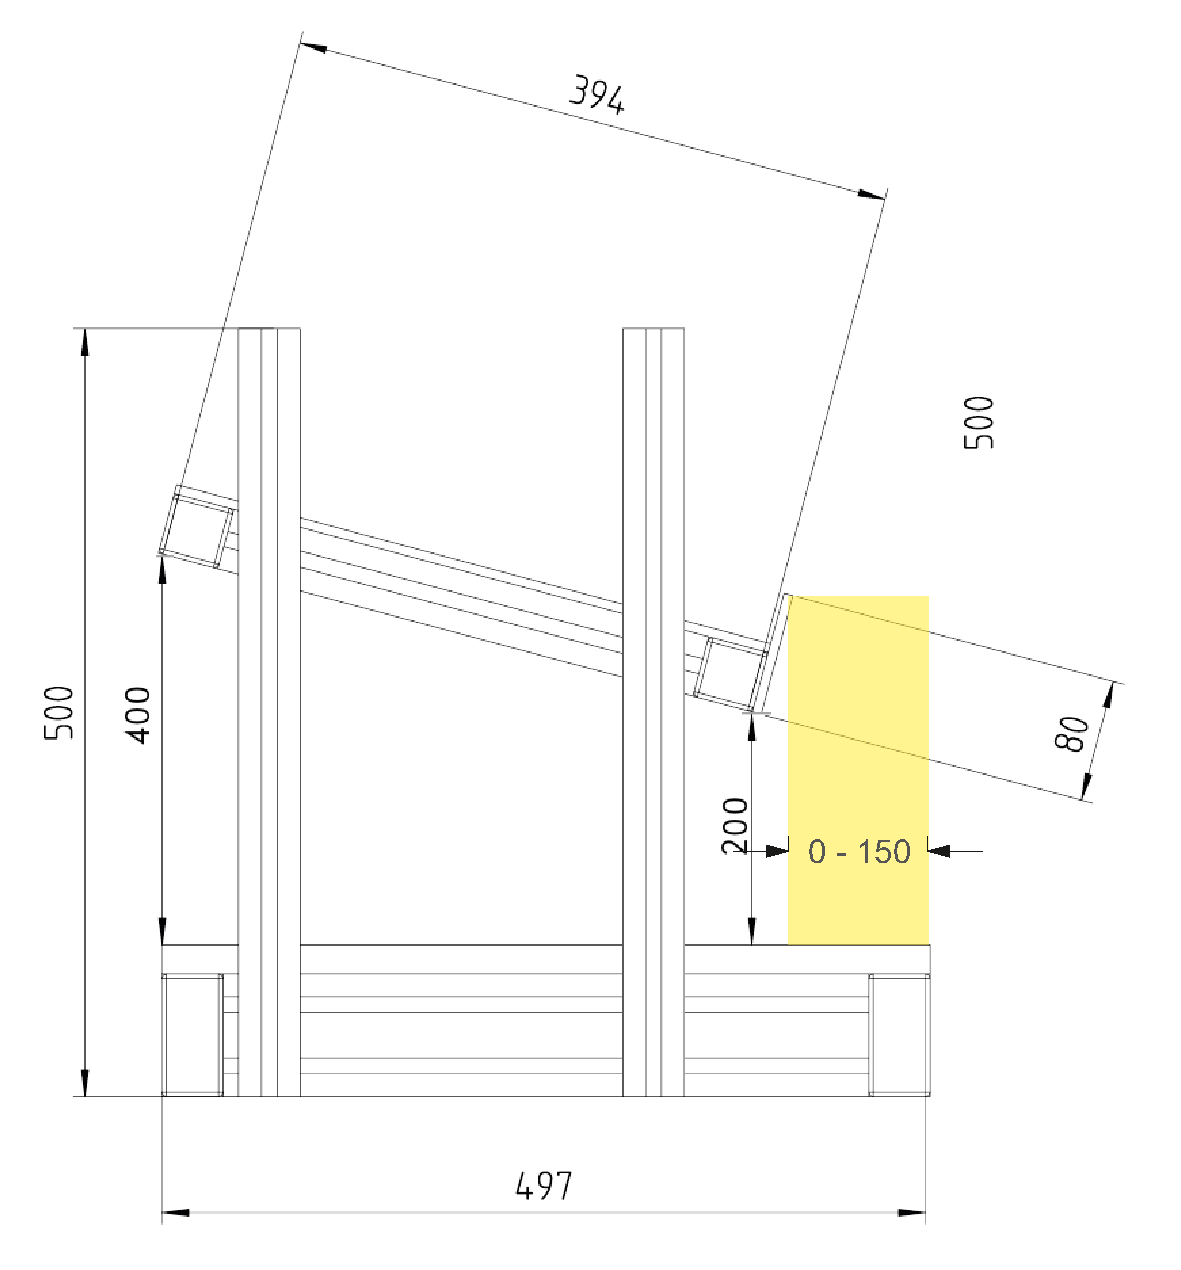
\includegraphics[width=0.375\textwidth ]{./images/shelfUpdate.pdf} }
	\caption{Exemplary shelf and generic technical drawing.}%
	\label{fig:shelf}
\end{figure}


\subsection{Rotating Tables}\label{sec:Rotating Table}
The integration of Rotating Tables into tests is according the table \ref{fig:test_specifications_instance}.  A Rotating Table as depicted in Figure~\ref{fig:rottable} is used for these tests. The Objects placement is the same like in section \ref{ssec:ManipulationZone}, so the maximal depth for Objects is $20 \si{\centi\meter}$ and there is gap of $2\si{\centi\meter}$ to the border of the Rotating Table.


The height of the Rotating Table should be not lesser than $8\si{\centi\meter}$ and not be more than $12\si{\centi\meter}$. The diameter of the Rotating Table should be not lesser than $50\si{\centi\meter}$ and not more than $100\si{\centi\meter}$. The Rotating Table has to have a white surface colour. The rotating speed of the table depends on the diameter so that the Objects speed is able to vary between $5 \si{\centi\meter\per\second} \le v_{object} \le 20 \si{\centi\meter\per\second}$. This has to be adjusted by the referees before a team starts its run to a fixed value (some small variations in boarders of  technical feasibility are allowed). This is changed after each run type to another random chosen value in this range. During the run of a team the speed is static and each team will have the same table speed. Example: For a Rotating Table with diameter $d_{table}=1\si{\meter}$, Objects are placed on a grasp region with the diameter $d_{object}=0.8\si{\meter}$ with $\omega_{table} = \frac{2 \cdot v_{objects} }{d_{grasp}}=\frac{2 \cdot 0.2}{0.8}=0.5\si{\radian\per\second}$ and with $n_{table}=\frac{\omega_{table}}{2 \cdot \pi}=\frac{0.5}{2 \cdot \pi}$ the minimum rotational speed of the Rotating Table $n_{table}= 0.0796 \si{\per\second}$ (rounds per second) can be calculated.  

\begin{figure}[h!]
	\centering
	\subfloat[A Rotationg table with some Objects.]{%
		\includegraphics[width=0.375\textwidth,angle=0 ]{./images/rotating_table.jpg}%
	}%
	\hspace{0.05\textwidth}
	\subfloat[Technical draw of Rotating table.]{%
		\includegraphics[width=0.375\textwidth ]{./images/rotating_table_schematic.pdf}
	}
	\caption{Exemplary Rotating table and generic technical drawing.}%
	\label{fig:rottable}
\end{figure}


\subsection{Precision Placement Tables}\label{sec:Precision Placement}

The precision placement table as shown in Figure~\ref{fig:ppt_table} includes object-specific cavities tiles as shown in the Figure~\ref{fig:ppt_tiles}. It is based on a standard $10\si{\centi\meter}$ table described in Section~\ref{subsec: Tables}. For each object used in the test, there will be one specific cavity. The cavity has the dimension of the object plus a $2 \si{\milli\meter}$ offset for each dimension. At most five cavities are used in the test. The cavities are in an random order on the table and are located within the standard manipulation zone defined in Figure~\ref{fig:manipulation_zone}. One cavity tile has the dimensions of $140 \si{\milli\meter} \times 140 \si{\milli\meter} $. Placing five cavities on a standard $10\si{\centi\meter}$ table leaves a boarder of $5 \si{\centi\meter}$ on each side of the table. The additional decoy cavity tiles will be chosen by the referees. For the Precision Placement Table only the RoboCup@Work Object Set will be used.
\clearpage

\begin{figure} [h!]
	\begin{center}
		\subfloat[F20\_20]{\includegraphics[width = 2cm]{./images/ppt_F20.png}} \hspace{0.1cm}
		\subfloat[S40\_40]{\includegraphics[width = 2cm]{./images/ppt_S40.png}} \hspace{0.1cm} 
		\subfloat[M20\_100]{\includegraphics[width = 2cm]{./images/ppt_M20_100.png}}  \hspace{0.1cm}
		\subfloat[M20]{\includegraphics[width = 2cm]{./images/ppt_M20.png}}  \hspace{0.1cm}
		\subfloat[M30]{\includegraphics[width = 2cm]{./images/ppt_M30.png}}  \hspace{0.1cm}
		\subfloat[R20]{\includegraphics[width = 2cm]{./images/ppt_VR20.png}} \\
		\subfloat[F20\_20]{\includegraphics[width = 2cm]{./images/ppt_F20_v.png}}  \hspace{0.1cm}
		\subfloat[S40\_40]{\includegraphics[width = 2cm]{./images/ppt_S40_v.png}}   \hspace{0.1cm}
		\subfloat[M20\_100]{\includegraphics[width = 2cm]{./images/ppt_M20_100_v.png}} \hspace{0.1cm}
		\subfloat[M20]{\includegraphics[width = 2cm]{./images/ppt_M20_v.png}}  \hspace{0.1cm}
		\subfloat[M30]{\includegraphics[width = 2cm]{./images/ppt_M30_v.png}}  \hspace{0.1cm}
		\subfloat[R20]{\includegraphics[width = 2cm]{./images/ppt_VR20_v.png}} 
	\end{center}
	\caption{Illustration of horizontal (top row) and vertical (bottom row) cavities for the different kind of manipulation objects.}
	\label{fig:ppt_tiles}
\end{figure}



%\begin{figure} [h!]
%	\centering
%	\includegraphics[width= 0.4\textwidth ]{./images/ExampleCavity.jpg}
%	\caption{Example Cavity for F20\_B and G horizontal including $3\si{\milli\meter}$ boarder. }
%	\label{fig:exampleCavity}
%\end{figure}


\begin{figure}[h!]
	\centering

	\subfloat[The PPT platform including five cavity tile.]{%
	\includegraphics[width=0.45\textwidth ]{./images/ppt_plattform.jpg}
	}%
	\hspace{0.05\textwidth}
	\subfloat[Technical draw of Precision Placement table.]{%
		\includegraphics[width=0.45\textwidth ]{./images/PPTtable.pdf}
	}
	\caption{Exemplary Precision Placement table and generic technical drawing.}%
	\label{fig:ppt_table}
\end{figure}



\subsection{Arena Layout}
\label{ssec:ArenaGeneral}

%\textbf{Layout:}
The arena is a static 2D environment consisting of Walls, Tables and Obstacles etc. with a size of atleast 10 m$^2$ and not more than 120 m$^2$. 
An example layout is shown in fig. \ref{fig:arena_example}.

\begin{figure} [h!]
	\centering
	\includegraphics[width= 1\textwidth ]{./images/general_rules/arena_example.jpg}
	\caption{An exemplary setup of a \RCAW environment.}
	\label{fig:arena_example}
\end{figure}

Layouts may include rooms and hallways to create more realistic scenarios.
Service Areas (see section \ref{sec:Service_Areas}) mark the locations for robots to perform tasks.
Each requested Service Area must be accessible via atleast one path of $80\si{\centi\meter}$ width.

\begin{figure} [h!]
	\centering
	\includegraphics[width= 0.8\textwidth ]{./images/general_rules/arena_map_annotated}
	\caption{Annotated 2D map of the environment in fig. \ref{fig:arena_example}}
	\label{fig:arena_map_annotated}
\end{figure}

Each competition has a new and unique layout designed by the actual TC members.
It should feature:
\begin{itemize}
	\item Area 10 m$^2$ - 120 m$^2$
	\item Minimum distance between arena elements at least $80\si{\centi\meter}$ 
	\item Widespread Service Areas entailing robot movements
	\item Multiple paths between Service Areas
	\item START and FINISH area
\end{itemize}

\clearpage
\textbf{START and FINISH area:}
\label{subsubsec: Start and Goal Area}

One or two parts of the arena are separated with marking Tape and considered as START and FINISH area. The START and FINISH area can be the same or two independent areas. The robot may leave the START area and enter the FINISH area only once. The START/FINISH area is leaved/entered when the robot completely cross the corresponding Marking Tape. In figure \ref{fig:tapeconfig} an exemplary Tape configuration is shown. As soon as the robot enters the FINISH area or re-enters the START area the run ends. The FINISH area counts as a Service Area and reaching the FINISH area gives additional points. 

\begin{figure} [h!]
	\begin{center}
		\includegraphics[width= 0.6\linewidth]{./images/arena/tabes.pdf}
	\end{center}
	\caption{Exemplary tape configuration: black lines are physical walls, red white dashed lines are virtual walls, yellow black dashed lines are barrier tape and green lines are marking tape}
	\label{fig:tapeconfig}
\end{figure}




\textbf{Referee Zone}

The arena is enclosed by a padded strip of 1m. This area is reserved for the referees to enable them to move freely while judging a robot's performance. See section \ref{sec: teams and roles}.


\clearpage

\section{Service Areas}
\label{sec:Service_Areas}
A Service Area indicates a location for a robot where tasks (e.g. picking or placing Objects) have to be performed.
\subsection{General} 
\label{subsec:Service_Areas_General}


Such a location is usually a Table with a flat white top (see fig. \ref{fig:arena_example}), commonly referred to as Workstation (only in a case of a normal Table), but can also be a Rotating Table, Shelf, Precise Placement station or any other type needed for a specific task.
In order to successfully reach a Service Area, robots must position themselves in front of the Service Area in a way that allows manipulation of the Objects of interest and the robot has to stand still. To enable robots to reach such a position, a rectangular area with $80\si{\centi\meter}$ width must be kept free of Obstacles (see fig. \ref{fig:arena_service_area_free}). 

\begin{figure} [h!]
	\centering
	\includegraphics[width= 0.8\textwidth ]{./images/general_rules/arena_service_area_free_space}
	\caption{Free Space in front of a Service Area}
	\label{fig:arena_service_area_free}
\end{figure}

The arena layout must define where the "front" of a table is.
Figure \ref{fig:arena_map_annotated} gives an example for the definition of the position of each Service Area, marking them as WSx (Workstation x), SHx (Shelf x), PPx (Precise Placement x)and RTx (Rotating Table x). The orientation only indicates the direction of the Service Area. It does not specify the robot's heading, which may be chosen by teams according to their individual robot design.

Tables that includes Service Areas which can be used from both sides (see fig. \ref{fig:arena_example}) are defined as two seperate workstations (e.g. WS5 \& WS6). However, manipulation of theses Service Area requires the robot to have its center in the rectangular area defined in fig.~\ref{fig:arena_service_area_free}. This means that manipulation of the opposite Service Area is NOT allowed (see \ref{ssec:ManipulationZone}), even though it would be physically possible.

This rule also applies to the two positions for the Rotating table (RT1 and RT2).
This makes smaller physical layouts possible that still provide the ability to create complex navigation challenges due to the amount of locations to visit.


\subsection{Arbitrary Surfaces and Decoys}
\label{subsec:Arbitrary_Surfaces_and_Decoys}

In order to make the operating environment more realistic, the Service Areas may contain different kinds of Arbitrary Surfaces (Figure \ref{fig:ast_surface_example}) with industrial items as Decoys (Figure \ref{fig:ast_example}). The Arbitrary Surfaces don't have to be fixed mounted at the Service Areas. Examples of Arbitrary Surfaces can be different wood pattern, grass, alufoil, plexiglas etc. The integration of Arbitrary Surfaces and Decoys into tests is according the table \ref{fig:test_specifications_instance}.


\begin{figure}[h!]
	\centering
	\subfloat[]{\includegraphics[width=.23333\textwidth]{./images/Arbitrary_Surface_rug}}
	\hspace{.05\textwidth}
	\subfloat[]{\includegraphics[width=.23333\textwidth]{./images/Arbitrary_Surface_wood}}
	\hspace{.05\textwidth}
	\subfloat[]{\includegraphics[width=.23333\textwidth]{./images/Arbitrary_Surface_grass}}\\
	\subfloat[]{\includegraphics[width=.23333\textwidth]{./images/Arbitrary_Surface_fake_wood_1}}
	\hspace{.05\textwidth}
	\subfloat[]{\includegraphics[width=.263333\textwidth]{./images/Arbitrary_Surface_fake_wood_2}}
	\caption{Examples of arbitrary surfaces used for Service Areas.}
	\label{fig:ast_surface_example}
\end{figure}

\begin{figure}[h!]
	\begin{center}
		\subfloat[]{\includegraphics[width=.375\textwidth]{./images/realisticWorkingDeskI.jpeg}}
		\hspace{.05\textwidth}
		\subfloat[]{\includegraphics[width=.375\textwidth]{./images/realisticWorkingDeskII.jpeg}}
	\end{center}
	\caption{Examplary configuration of the working desks including objects and decoys.}
	\label{fig:ast_example}
\end{figure}

Placement of Decoys and arbitrary surfaces are done by the referees. Decoys could be any kind of object (tools, hardware, small electrical devices) but also standard objects from the rule book defined in section~\ref{ssec:ManipulationObjects} can be used. Figure~\ref{fig:ast_example} shows some examples. 



\subsection{Containers}
As in many industrial settings, the \RCAW environment may be equipped with several Containers (see Figure~\ref{fig:containers}). The Containers are defined as industrial plastic stacking boxes size 2B, outer dimensions: $135 \times 160 \times 82  \si{\milli\meter}$, usable dimensions: $120 \times 125 \times 65  \si{\milli\meter}$  in red ca. RAL 3020 and blue ca. RAL 5015.
% \href{https://www.amazon.de/gp/product/B0062TUUOE/ref=ppx_yo_dt_b_asin_title_o01_s00?ie=UTF8&psc=1}{example Container from amazon} (visited Januar 2022). 
They can store any kind of Object defined in Section~\ref{ssec:ManipulationObjects}. Robots are supposed to place previously grasped Objects into containers. 
(Grasping from containers might be included in future competitions.) Several Containers can be present in the environment and are always associated with a Service Area. That means that the Container itself will be placed within the manipulation zone defined in Section~\ref{ssec:ManipulationZone}.
It is also possible that more than one Container is placed at a single Service Area, but not multiple Containers of the same color.
The constraints defined in Section~\ref{ssec:ManipulationZone} apply also to the Containers.
Currently, a Container itself does not need to be manipulated or transported by the robot. The position of the Containers will be decided by the referees before every run type.

\begin{figure} [h!]
	\begin{center}
		\subfloat[blue]{\includegraphics[width= 0.375\textwidth]{./images/container_blue.jpg}} 
		\hspace{0.05\textwidth}
		\subfloat[red]{\includegraphics[width= 0.375\textwidth]{./images/container_red.jpg}}
	\end{center}
	\caption{Containers can be used for grasping Objects out or placing Objects into them.}
	\label{fig:containers}
\end{figure}


\section{Objects} 
\label{ssec:ManipulationObjects}

The Objects in \RCAW include a wide range of Objects relevant in industrial applications of robotics. They eventually cover any raw material, (semi-)finished parts or products as well as tools and possibly operating materials required for manufacturing processes. Object types are selected by the TC and shall vary in complexity due to different shapes, colors and uses of objects. Currently there are three sets of Objects used in the competition: Basic, Advanced and April Tagged. The following sections provide details about those sets. The exact appearance of the object used in the competition can slightly vary due to availability, e.g. different coating colors for some standard parts.



%TODO: Still need this or can we remove it with introduction of new object set?
%
%Additionally, a set of so called RoCKIn objects is used in the competition (see table~\ref{tab:manipulation_objects_rockin}). 
%These parts build a drive train of a KUKA youbot and might be used for assembly tasks.
%\textbf{REMARK:} Due to poor availability of the original RoCKin object set, teams are allowed to to use a set of 3D printed copies. The material used for fabrication has to be in standard grey/silver colour using fine quality settings and PLA as printing material. 
%An example is given with PLA Silver (ca. RAL 9006), thickness 1.75 or 2.85, not specified in detail.

%\href{https://www.amazon.de/-/en/TINMORRY-1-75mm-Filament-Printer-Spool/dp/B089YX78N5/ref=sr_1_6?crid=ZTL2O0EL3B3B&keywords=pla%2Bfilament%2Bgrau%2Bral%2B9006&qid=1641982915&s=industrial&sprefix=pla%2Bfilament%2Bgrau%2Bral9006%2Cindustrial%2C114&sr=1-6&th=1 }{example material from amazon} (visited Januar 2022). 
%Figure~\ref{fig:RoCKIn_printed} shows an example set of the printed RoCKIn Objects created using fused filament fabrication (FFF) printing. 


% as shown in  and . Objects of one kind can slightly vary e.g. considering the surface and coating colour. 

%RoCKIn Objects are spare parts from the KUKA you-bot platform often used in the competition, due to the fact that the KUKA you-bot and the RoCKIn Objects are not longer produced in future those Objects will be replaced with other standard parts used in industry as shown in Section~
%\ref{sec:new_objects}. 


\subsection{Basic Object Set}

The Basic Object Set includes standard profile rails, screws and nuts with various sizes and masses.
% (see table~\ref{tab:manipulation_objects}).

\newcommand{\imageView}[1]{\includegraphics[width=2cm, valign=c]{#1}}
\newcommand{\rowpadding}{0.4cm}
\setlength\extrarowheight{\rowpadding}


\begin{table}[h!]

\begin{tabular}{|c|c|c|c|m{8cm}|}
\hline
ID & Object & Symbolic Description & Mass & Details \\
\hline

\texttt{1} & \imageView{./images/F20_20_B.jpg} & \texttt{F20\_20\_B} & 49 g & Small aluminium profile \newline
 Coating/Colour: black anodized\newline
 Size: $20 \times 20 \times 100 mm$ \\ [\rowpadding]
\hline

\texttt{2} & \imageView{./images/F20_20_G.jpg} & \texttt{F20\_20\_G} & 49 g & Small aluminium profile \newline
 Coating/Colour: gray anodized\newline
 Size: $20 \times 20 \times 100 mm$ \\ [\rowpadding]
\hline

\texttt{3} & \imageView{./images/S40_40_B.jpg} & \texttt{S40\_40\_B} & 186 g & Large aluminium profile\newline
 Coating/Colour: black anodized\newline
 Size: $40 \times 40 \times 100 mm$ \\ [\rowpadding]
\hline

\texttt{4} & \imageView{./images/S40_40_G.jpg} & \texttt{S40\_40\_G} & 186 g & Large aluminium profile \newline
 Coating/Colour:  gray anodized\newline
 Size: $40 \times 40 \times 100 mm$ \\[\rowpadding]
\hline

\texttt{5} & \imageView{./images/M20_100.jpg} & \texttt{M20\_100} & 296 g & Screw\newline
 ISO4014, DIN 931, EU 24014 \newline
 Coating/Colour: blank, black burnished \newline
 Size: M$20\times 100$ \\ [\rowpadding]
\hline

\texttt{6} & \imageView{./images/M20.jpg} & \texttt{M20} & 56 g & Small nut\newline
 ISO4032, DIN934, EU 24032  \newline
 Coating/Color: blank, black burnished \newline
 Size: M20 \\ [\rowpadding]
\hline

\texttt{7} & \imageView{./images/M30.jpg} & \texttt{M30} & 217 g & Large nut\newline
 ISO4032, DIN934, EU 24032  \newline
 Coating/Color: blank, black burnished \newline
 Size: M30 \\ [\rowpadding]
 \hline
\end{tabular}
\caption{\RCAW Object set.}
\label{tab:manipulation_objects}
\end{table}



\clearpage
%\subsection{RoCKIn Object Set}
%
%\subsubsection{Original Set}
%
%
%\begin{table}[h!]
%\begin{tabular}{|c|c|c|c|m{6cm}|}
%\hline
%ID & Object & Symbolic Description & Mass & Details \\
%\hline
%
%\texttt{8} & \imageView{./images/bearingBoxA.jpg} & \texttt{Bearing\_Box} & 102 g & Bearing box\newline
% Height: 25 mm \newline
% Width: 45 mm \newline
% Length: 50 mm \newline
% Inner diameter: 32 mm \\ [\rowpadding]
%\hline
%
%\texttt{9} & \imageView{./images/bearing.jpg} & \texttt{Bearing} & 42 g & Bearing\newline
% Height: 13 mm \newline
% Inner diameter: 15 mm \newline
% Outer diameter: 32 mm \\ [\rowpadding]
%\hline
%
%\texttt{10} & \imageView{./images/axis.jpg} & \texttt{Axis} & 40 g & Axis\newline
% Diameter: 27 mm \newline
% Length: 96 mm \\ [\rowpadding]
%\hline
%
%\texttt{11} & \imageView{./images/distanceTube.jpg} & \texttt{Distance\_Tube} & 5 g & Distance tube\newline
% Height: 10 mm \newline
% Inner diameter: 28 mm \newline
% Outer diameter: 32 mm \\ [\rowpadding]
%\hline
%
%\texttt{12} & \imageView{./images/motor.jpg} & Motor & 20 g & Motor\newline
% Diameter: 42 mm \newline
% Length: 87 mm \\ [\rowpadding]
%\hline
%
%\texttt{13} & \imageView{./images/R20.jpg} & \texttt{R20} & 14 g & Plastic tube\newline
%Inner diameter: 20 mm \newline
%Outer diameter: 30 mm \newline
%Length: 45 mm \\ [\rowpadding]
%\hline
%%\imageView{./images/V20.jpg} & \texttt{V20} & 14 g & Inner diameter: 20 mm \newline
%%Outer diameter: 30 mm \newline
%%Length: 45 mm \\
%%\hline
%\end{tabular}
%\caption{RoCKIn Object set.}
%\label{tab:manipulation_objects_rockin}
%\end{table}
%}
%
%\clearpage
%\subsubsection{Printed Set}
%
%
%\begin{figure}[h!]
%	\begin{center}
%		\subfloat[]{\includegraphics[width=0.8\textwidth]{./images/rockingPrinted1.jpg}}
%		\vspace{0.05\textwidth}
%		\subfloat[]{\includegraphics[width=0.8\textwidth]{./images/rockingPrinted2.jpg}}
%	\end{center}
%	\caption{Examplary 3D printed RoCKIn Objects (bearing box, bearing, axis, distance\_tube, motor, plastic tube R20). Material:  PLA silver ( ca. RAL 9006), 2.85mm. Printer: Ultimaker 3 extended. Printer settings: fine}
%	\label{fig:RoCKIn_printed}
%\end{figure}



\clearpage
\subsection{Advanced Object Set}


For 2023, the RoCKIn object set (see 2022 rulebook or previous ones) is replaced by a selection of better available parts for a drive train, as well as some tools (see Section~\ref{sec:new_objects}). The new object set was introduced in a technical challenge in 2022 and is called Advanced Object Set.

\begin{table}[h!]
	\begin{tabular}{|c|m{2cm}|c|c|m{8cm}|}
		\hline
		ID & Object & Symbolic Description & Mass & Details \\
		\hline
%%%%%%%%%%%%%
		\texttt{20} & \imageView{./images/newObjects/welle3d.jpg} \newline
		\imageView{./images/newObjects/welleSchematic.JPG}
		& \texttt{Axis2} & 180 g & Steel axis \newline
		Misumi: SFUB25-25-F28-P17-T15-S10-Q20 \newline
		Coating/Colour: blank, black burnished \newline
		Length: 68 mm \newline
		Diameter: 17mm, M20 \newline
		%see Figure~\ref{fig:welle2Schematic} \newline
		
		\href{https://de.misumi-ec.com/vona2/detail/110302635710/?CategorySpec=00000146753%3a%3ab%2cc}{Misumi} (visited Januar 2022)\\

			\hline
%%%%%%%%%%%%
		\texttt{21} & \imageView{./images/newObjects/bearing2.JPG} & \texttt{Bearing2} & 100 g & Bearing \newline 
		SKF YAR203-2F\newline
		Coating/Colour: gray \newline
		Useable with housing\newline
		\href{https://www.skf.com/sg/products/rolling-bearings/ball-bearings/insert-bearings/productid-YAR%20203-2F}{SKF}  (visited Januar 2022)\\
		\hline
%%%%%%%%%%%%				
		\texttt{22} & \imageView{./images/newObjects/housing.JPG} & \texttt{Housing} & 60 g & Housing \newline 
		SKF P40\newline
		Coating/Colour: gray \newline
		Useable with bearing\newline
		\textbf{Remark:} needs two hex socket screw M8x10 (ISO 4762, DIN 912) and two M8 nuts (ISO 4032, DIN 934) \newline
		\href{https://www.skf.com/sg/products/mounted-bearings/ball-bearing-units/pillow-block-ball-bearing-units/productid-P%2040}{SKF}  (visited Januar 2022)\\
		\hline
%%%%%%%%%%%%	
		\texttt{23} & \imageView{./images/newObjects/motor.JPG} & \texttt{Motor2} & 350g & Motor 755\newline
		Coating/Colour: gray \newline
		Size: $66.7 \times 42.0 \si{\milli\meter}$\newline
		Diameter: $d_{axis}=5\si{\milli\meter}$, $l_{axis}=10\si{\milli\meter}$ \newline
		\href{https://www.amazon.de/EsportsMJJ-12V-36V-3500-9000Rpm-Drehmoment-Hochleistungsmotor/dp/B075D85KVV}{Amazon}  (visited Januar 2022)\\
		\hline
%%%%%%%%%%%%					
		\texttt{24} & \imageView{./images/newObjects/FlangedResinCollar.JPG} & \texttt{Spacer} &  & Flanged Spacer\newline
		Misumi CLJHJ25-30-70  \newline
		Coating/Colour: white \newline
		Size: $70\si{\milli\meter}$\newline
		Diameter: $d_{inner}=25\si{\milli\meter}$, $d_{outer}=30\si{\milli\meter}$ \newline
		\href{https://us.misumi-ec.com/vona2/detail/110300236450/?curSearch=%7b%22field%22%3a%22%40search%22%2c%22seriesCode%22%3a%22110300236450%22%2c%22innerCode%22%3a%22%22%2c%22sort%22%3a1%2c%22specSortFlag%22%3a0%2c%22allSpecFlag%22%3a0%2c%22page%22%3a1%2c%22pageSize%22%3a%2260%22%2c%2200000042362%22%3a%22mig00000001500952%22%2c%2200000042368%22%3a%22b%22%2c%22jp000157843%22%3a%22mig00000000344081%22%2c%22jp000157846%22%3a%22mig00000001417174%22%2c%22jp000157851%22%3a%22mig00000000344088%22%2c%2200000334029%22%3a%2230%22%2c%2200000334032%22%3a%2270%22%2c%22typeCode%22%3a%22CLJHJ%22%2c%22fixedInfo%22%3a%22MDM0000085422111030023645020110476153310093415426696895%7c14%22%7d&Tab=preview}{Misumi}  (visited Januar 2022)\\
						\hline

\end{tabular}
\caption{Advanced Object Set}
\label{tab:new_objects1}
\end{table}


\begin{table}[h!]
	\begin{tabular}{|c|m{2cm}|c|c|m{8cm}|}
		\hline
		Object & Symbolic Description & Mass & Details \\
		\hline
		%%%%%%%%%%%%
		\texttt{24} & \imageView{./images/newObjects/weraScrewdriver.jpg} & \texttt{Screwdriver } & 19g & WERA 352 \newline
		Ball end screwdriver,hexagon socket screws\newline
		Coating/Colour: black/green \newline
		Size: $181\si{\milli\meter}$\newline
		Diameter: $d_{tip}=2.5\si{\milli\meter}$\newline
		Code: 05138070001\newline
		\href{https://www.amazon.de/Wera-05138070001-352-Sechskant-Kugelkopf-Schraubendreher-2-5/dp/B00154ZWFI?th=1}{Amazon}  (visited Januar 2022)\\
		\hline
		%%%%%%%%%%%%			
		\texttt{25} & \imageView{./images/newObjects/weraWrench.jpg} & \texttt{Wrench } & ca. 72g & WERA Jocker 6000, 8mm \newline
		Ratcheting combination wrenches\newline
		Coating/Colour: silver/grey/pink \newline
		Size: ca. $144\si{\milli\meter}$\newline
		Diameter: $d_{max}=20\si{\milli\meter}$\newline
		Code: 05073268001\newline
		\href{https://www.amazon.de/Wera-05073268001-Joker-Maul-Ringratschen-Schl%C3%BCssel/dp/B00BT0GBMG?th=1}{Amazon} (visited Januar 2022)\\
		\hline
		%%%%%%%%%%%%
		\texttt{26} & \imageView{./images/newObjects/hsscoDIN338metaldrill.jpg} & \texttt{Drill } & ca. 10g & Bosch Drill HSS-Co DIN338  \newline
		Drill\newline
		Coating/Colour: gold/ Cobalt alloy \newline
		Length: ca. $151\si{\milli\meter}$\newline
		Diameter: $d_{max}=13\si{\milli\meter}$\newline
		Code: 3165140382724 \newline
		\href{https://www.amazon.com/Bosch-2609255086-Metal-Drill-HSS-Co/dp/B0071OSFQY}{Amazon} (visited Januar 2022)\\
		\hline
		%%%%%%%%%%%
		\texttt{27} & \imageView{./images/newObjects/weraAllenKey.jpg} & \texttt{AllenKey } & ca. 10g & Wera Allen Key 8mm,\newline
		3950 PKL L-key, metric, stainless\newline
		Coating/Colour: silver \newline
		Length: ca. $195\si{\milli\meter} \times 37\si{\milli\meter}$\newline
		Diameter: $d_{max}=8\si{\milli\meter}$\newline
		Code: 05022708001 \newline
		\href{https://www.amazon.co.uk/Wera-WER022708-Hexagon-Keys-Multi-Colour/dp/B00A8QXTNG}{Amazon} (visited Januar 2022)\\
		\hline
		%%%%%%%%%%%
	
\end{tabular}
\caption{\RCAW New set of manipulation objects (tool set).}
\label{tab:new_objects2}
\end{table}

\clearpage


\subsection{April Tagged Object Set}
\label{ssec: April Tagged Object Set}

For the season 2023 and onwards, 3D printed cubes marked with April tags might be used in the competition. 
This should allow teams to focus on other areas than object recognition by simplifying the detection of Objects. 
These cubes will be called April Tag Tagged Cubes (ATTC) in the following.

The April Tags used in \RCAW measure $40 \si{\milli\meter} \times 40 \si{\milli\meter}$ and have an encoding taken from the \textit{36h11} April Tag family, including a 1bit black and 1bit white border as shown in fig. \ref{fig:singleAprilTag}. 


\begin{figure}[h!]
	\centering
	\includegraphics[width= 0.4\textwidth ]{./images/singleAprilTAG42.png}
	\caption{Example of an April Tag with the ID 42. Encoding is from the 36h11-April Tag Family.}
	\label{fig:singleAprilTag}
\end{figure}

All the used April Tag ID numbers will fit to the ID numbers used by the AtWork Commander in the \href{https://github.com/robocup-at-work/atwork-commander/blob/master/atwork_commander_msgs/msg/Object.msg}{atwork\_commander\_msgs/msg/Object.msg}. 
%
%uint16 EMPTY = 0
%
%# atwork
%uint16 ATWORK_START = 11
%uint16 F20_20_B = 11
%uint16 F20_20_G = 12
%uint16 S40_40_B = 13
%uint16 S40_40_G = 14
%uint16 M20_100 = 15
%uint16 M20 = 16
%uint16 M30 = 17
%uint16 R20 = 18
%uint16 ATWORK_END = 19
%
%# rockin
%uint16 ROCKIN_START = 21
%uint16 BEARING_BOX = 21
%uint16 BEARING = 22
%uint16 AXIS = 23
%uint16 DISTANCE_TUBE = 24
%uint16 MOTOR = 25
%uint16 ROCKIN_END = 26
%
%# container
%uint16 CONTAINER_START = 31
%uint16 CONTAINER_RED = 31
%uint16 CONTAINER_BLUE = 32
%uint16 CONTAINER_END = 33
%
%# cavity
%uint16 CAVITY_START = 41
%uint16 F20_20_H  = 41
%uint16 F20_20_V  = 42
%uint16 F20_20_F  = 43
%uint16 S40_40_H  = 44
%uint16 S40_40_V  = 45
%uint16 S40_40_F  = 46
%uint16 M20_H     = 47
%uint16 M20_V     = 48
%uint16 M20_F     = 49
%uint16 M20_100_H = 50
%uint16 M20_100_V = 51
%uint16 M20_100_F = 52
%uint16 M30_H     = 53
%uint16 M30_V     = 54
%uint16 M30_F     = 55
%uint16 R20_H     = 56
%uint16 R20_V     = 57
%uint16 R20_F     = 58
%uint16 CAVITY_END = 59 


\subsubsection{ATTC as Manipulation Objects}

The standard ATTC measures $42\si{\milli\meter} \times 42\si{\milli\meter} \times 42 \si{\milli\meter}$ and has slightly rounded edges, similar to the shape of aluminum profile rails. On the top there is a $1\si{\milli\meter}$ deep cavatie ( $40.5\si{\milli\meter} \times 40.5\si{\milli\meter}$) to place the individual April Tag. It is manufactured by 3D printing using PLA filament of any color. The april tag is glued to the top side of the ATTC and is encoded with an ID matching one of the objects.
The exact design and size is specified in fig. \ref{fig:cubeObject} and can be downloaded from the official league repository: \href{https://github.com/robocup-at-work/rulebook/tree/alpha_2023/images}{3D STL file of manipulation Cube.}
The sides are marked with the ID in numeric numbers to make the cubes also identifyable by humans.

\begin{figure}[h!]
	\centering
	\subfloat[April Tag Tagged Cube (ATTC), including overall dimensions.]{\includegraphics[width=0.375\textwidth ]{./images/AprilTags/AprilTagCube2023_2.png}}
	\hspace{0.05\textwidth}
	\subfloat[Detailed dimensions of the ATTC cavaty to fix a certain April Tag.]{ \includegraphics[width=0.375\textwidth ]{./images/AprilTags/AprilTagCube2023_1.png} }
	\caption{3D construction of the ATTC as manipulation object.}%
	\label{fig:cubeObject}
\end{figure}

\subsubsection{Tagged Targets}

Target objects, such as a precise placement cavity or a container, might also be marked with an April Tag.

For the PP cavaty tiles, one design will be used for all ATTC with any object ID. The design foresees a matching hole and two square cut-outs where tagged plates can be inserted. Additional to the April Tag also the April Tag ID will be shown on the tile.
The ID used matches the ID used in the Atwork Commander so it should also mach with the correct ATTC.
See the schematics shown in fig. \ref{fig:cubeObjectTile} for details. 

\begin{figure}[h!]
	\centering
	\subfloat[ATTC cavity tile, including overall dimensions.]{\includegraphics[width=0.375\textwidth ]{./images/AprilTags/CubeTile2023_2.png}}
	\hspace{0.05\textwidth}
	\subfloat[Detailed dimensions of the ATTC tile April Tag cavatie.]{ \includegraphics[width=0.375\textwidth ]{./images/AprilTags/CubeTile2023_1.png} }
	\caption{3D construction  of the ATTC Precision Placement cavaty tile.}%
	\label{fig:cubeObjectTile}
\end{figure}

Containers get an April tag glued onto the inside of the bottom surface with centric placement as shown in fig. \ref{fig:redContainerTagged}.

\begin{figure}[h!]
	\centering
	\includegraphics[width= 0.5\textwidth ]{./images/AprilTags/container_redTAG.png}
	\caption{Example of a red container, tagged with the April Tag ID: "31".}
	\label{fig:redContainerTagged}
\end{figure}


\subsubsection{April Tags}
April Tags can be easy generated. The usage of any ROS package to identify the April Tag is allowed. For example the \href{http://wiki.ros.org/apriltag_ros}{April Tag ROS package} can easy be adapted to be used within the competition. Example April Tags out of the April Tag Family  36h11 are shown in fig. \ref{fig:AprilTagExamples}. 


\begin{figure}[h!]
	\centering
	\includegraphics[width= 0.8\textwidth ]{./images/AprilTags/apriltags0to26.png}
	\caption{Examples of April Tags with $0 \le \mathrm{April Tag ID} \le 26$.}
	\label{fig:AprilTagExamples}
\end{figure}




\subsection{Manipulation Zone} \label{ssec:ManipulationZone}
The manipulation zone defines the area where Objects can be placed. Thereby, the following constraints need to be satisfied:
\begin{itemize}
	\item The maximum depth of the manipulation zone from the front of the service area to the end of the manipulation zone is $20\si{\centi\meter}$.
	\item The minimum distance between Objects to each other is $2\si{\centi\meter}$.
	\item The minimum distance of the beginning of the manipulation zone to a Wall is $10\si{\centi\meter}$.
	\item There as an offset of $2\si{\centi\meter}$ from the border of the Service Area to the manipulation zone.
\end{itemize}
Note, the constraints do not permit, that Objects can be partially occluded dependent on the viewpoint.

For the placement of Objects the following terms are used:

\begin{itemize}
	\item Position: point within 2D coordinate system of a Manipulation Zone,
	\item Rotation: rotation around vertical axis of a Manipulation Zone,
	\item Orientation: rotation around horizontal axes of a Manipulation Zone, i.e. whether the Object is standing upright or lying on its side
	\item Pose: combination of position, rotation and orientation.
\end{itemize}
\begin{figure} [h!]
	\centering
	\includegraphics[width=0.8\textwidth ]{./images/manipulation_zone2023.pdf}
	\caption{Manipulation zone: the green color indicates the area where Objects can be placed on a Service Area by the referees.}
	\label{fig:manipulation_zone}
\end{figure}












\chapter{Tests}

% !TEX root = ../Rulebook.tex

The actual competition contains a set of so-called tests. 
A test is specified in terms of it's purpose and focus, environment features and eventually manipulation objects involved. Further, a concrete specification of the task is given and the rules to be obeyed. 

Each test has different variability dimensions. That is, which objects to be manipulated, how many locations to visit, from which height to grasp etc. These dimensions are described in Section~\ref{sec:TestVariability} whereas in Section~\ref{sec:ScoringAndRanking} test instances for \YEAR are defined based on the general test description and instantiation of the variability dimensions. 

% !TEX root = ../Rulebook.tex
\newpage
\section{Basic Navigation Test}

\paragraph{Purpose and Focus of the Test}
The purpose of the \iaterm{Basic Navigation Test}{BNT} is to check whether the robots can navigate well in their environment, i.e. in a goal-oriented, autonomous, robust, and safe way.
\par
As the navigation problem is in the focus of robotics research for a long time and many approaches for solving it and its subtasks (like exploration, mapping, self-localization, path planning, motion control, and obstacle avoidance) exist, the focus of this test is to demonstrate that these approaches function properly on the robots used by the teams and in the environment defined by the test.
The arena used for this test contains all elements that affect or support navigation: walls, service areas, places, arena objects, wall markers, and floor markers. In addition, obstacles may be placed in the environment.
\par

\paragraph{Scenario Environment}
The arena used for this test contains all elements that affect or support navigation: walls, service areas, places, arena objects, wall markers, and floor markers. In addition, obstacles may be placed in the environment.

\paragraph{Manipulation Objects}
This test does not include any objects for manipulation.
\paragraph{Task}
For the navigation test, a single robot is used. The robot will be sent a task specification, which is a string containing a series of triples, each of which specifies a place, an orientation, and pause duration. The robot has to move to the places specified in the task string, in the order as specified by the string, orient itself according to the orientation given, cover a place marker, pause its movement for the time in seconds as specified by the pause length, and finally leave the arena through the gate.

The task specification consists of:

\begin{itemize}
	\item A destination location, e.g. \texttt{S1}, \texttt{D2}, \texttt{T7} or \texttt{U4}
	\item An orientation (\texttt{N}, \texttt{S}, \texttt{W}, \texttt{E})
	\item A duration in seconds
\end{itemize}

The duration is always set to 3 seconds in order to make validation easier for the referees.
%
% \subsection{Complexity Options}
%
% \subsubsection{Obstacle complexity (pick one):}
%
% \begin{itemize}
% 	\item Easy obstacles (bonus factor = +0.2): There are up to two obstacles in the arena.
% 	\item Medium obstacles (bonus factor =  +0.4): There are up to three obstacles in the arena and the placement of the obstacles is harder.
% \end{itemize}
%
%
% \subsubsection{Barrier Tape complexity (bonus factor = +0.4):}
% There are up to two barrier tape obstacles in the arena.
%
% \subsubsection{Navigation complexity (pick one):}
%
% \begin{itemize}
% 	\item Easy navigation (bonus factor = + 0.0): The place marker has to be covered in such a way by the robot that at least a part of the black area covered
% 	\item Medium navigation (bonus factor = + 0.1): The place marker has to be covered in such a way by the robot that at least a small part of the black area is covered the orientation must be correct, i.e. the robot must not deviate more than 45 deg.
% 	\item Hard navigation (bonus factor = + 0.2): The place marker has to be fully covered by the robot the orientation must be correct, i.e. the robot must not deviate more than 45 deg.
% \end{itemize}
%
%
\paragraph{Rules}
The following rules have to be obeyed:

\begin{itemize}
\item The order in which the teams have to perform will be determined by a draw.
\item After the team's robot enters the arena, it must move to the places given in the task specification and assume the orientation specified after the place. The robot may reach a destination by choosing any path.
\item The robot must visit the places in the order given by the task specification. It is possible to skip a place of the task specification and continue with the next one. In cases where the robot skipped one or multiple places there may be multiple possible matchings between places reached and places specified. In that case for calculating scores the matching is taken which leads to the highest score for the team.
\item A destination is counted as reached when the robot covers the place marker as much as the complexity level demands. The orientation must not deviate more than 45 deg.
\item When a destination is reached, the robot must stop its movement for the number of seconds specified by the break.
\item The time is stopped when the robot has completed the task and left the arena. If the team cannot complete the task within the designated time, the run will be stopped.
\end{itemize}
%
%
%
% \subsection{Scoring}
%
% \begin{itemize}
% \item The team will receive 50 points for reaching a destination correctly (place and orientation) as given in the task specification and provided it stops for the time specified.
% \item The team receives a penalty of –50 points each time the robot touches an obstacle, a wall, an arena object or a service area (i.e. any contact with the environment).
% \item 50 points are awarded for completing the task specification completely correct, i.e. visiting all destinations from the task specification according to position and orientation (according to the chosen complexity level) and finally leaving the arena.
% \item The reached points of a test will be multiplied with the complexity factor that belongs to the chosen complexity level.
% \end{itemize}


% !TEX root = ../Rulebook.tex


\section{Basic Manipulation Test}
\label{sec:Basic Manipulation Test}

The \iaterm{Basic Manipulation Test}{BMT} is the initial test for all robots in \RCAW .
The main focus is to demonstrate basic object recognition and manipulation capabilities of robots.

Therefore only two service areas will be used. Those service areas will be located near to each other, e.g. WS3 and WS4 in fig. \ref{fig:arena_example} and \ref{fig:arena_map_annotated}. One service area is used as the source location and one as the target location, meaning that all objects are initially placed on the source service area and have to be delivered to the target service area.

This test involves no arbitrary surfaces, decoy objects or obstacles.
The objects that have to be manipulated are pre-selected and will include one small grey alu (f20\_20\_g), one small nut (M20) and the bolt (M20x100). The placement and orientation of the objects will be random.

%However, a total number of 5 objects are placed on the source table.
%This means that the robot has to visit each service area atleast twice to complete the test successfully (transportation limit = 3, see \ref{ssec: Common Rules}).


%
%
%\paragraph{Purpose and Focus of the Test}
%The purpose of the \iaterm{Basic Manipulation Test}{BMT} is to demonstrate basic manipulation capabilities by the robots, like grasping, turning, or placing an object.
%\par
%The focus is on the manipulation and on demonstrating safe and robust grasping and placing of objects of different size and shape. Therefore, the number of service areas will be constraint to two, one source area and one target area, which are close to each other. 
%
%\paragraph{Scenario Environment}
%Additionally to environmental elements, different manipulatable objects will be placed on the specified service areas.
%
%\paragraph{Manipulation Objects}
%The manipulation objects used in this test are defined by the instances described in Table~\ref{tab:Instances}.
%
%\paragraph{Task}
%The task consists of a sequence of grasp and place operations, with a small base movement in between. The objective is to move a set of objects from one service area into another. To complete the task the source and the target destination have to be reached at least once.
%\par
%The task specification consists of:
%\begin{itemize}
%	\item[--] The specification of the initial place
%	\item[--] A source location, given as place (any one)
%	\item[--] A destination location, given as place (any one, but nearby the source location)
%	\item[--] A list of objects to manipulated from the source to the destination service area
%	\item[--] The specification of a final place for the robot
%\end{itemize}
%
%
%\paragraph{Rules}
%The following rules have to be obeyed:
%
%\begin{itemize}
%\item The order in which the teams have to perform will be determined by a draw.
%\item The robot will get the task specification from the referee box.
%\item A service area counts as successfully reached as defined in Section~\ref{ssec:Navigating}
%\item A manipulation object counts as successfully grasped as defined in Section~\ref{ssec:GraspingObjects}
%\item A manipulation object counts as successfully placed, if the robot has placed the object into the correct destination service area as described in Section~\ref{ssec:PlacingObjects}.
%\item  The run is over when the robot reached the final place or the designated time has expired.
%\item The score for this test will be calculated as defined in \ref{sec:ScoringAndRanking}.
%\end{itemize}
%



% !TEX root = ../Rulebook.tex
\newpage
\section{Basic Transportation Test}

\paragraph{Purpose and Focus of the Test}
The purpose of the \iaterm{Basic Transportation Test}{BTT} is to assess the ability of the robots for combined navigation and manipulation tasks \robin{as well as its task planning capabilities}. 
The robots have to deal with flexible task specifications, especially concerning information about object constellations in source and target locations, and task constraints such as limits on the number of objects allowed to be carried simultaneously, etc.

\paragraph{Scenario Environment}
The arena used for this test contains all elements as for the Basic Manipulation Test. Besides that all areas may contain objects.

\paragraph{Manipulation Objects}
The manipulation objects used in this test are defined by the instances described in Table~\ref{tab:Instances}.

\paragraph{Task}
\robin{\st{A single robot is used, which is initially positioned outside of the arena near a gate to the arena.}} The task is to get several objects from the source service areas (such as \texttt{SH02}, \texttt{WS09}, or \texttt{CB02}) and to deliver them to the destination service areas (e.g. \texttt{WS11} and \texttt{SH05}). \robin{\st{Robots may carry up to three objects simultaneously.}} 
\par
The task specification consists of two lists:
The first list contains for each service area a list of manipulation object descriptions. The descriptions are similar as those used for the Basic Manipulation Test. 
The second list contains for each destination service area a configuration of manipulation objects the robot is supposed to achieve. The configuration specification is similar as used in the Basic Manipulation Test. 

The term “line” in the task specification can be ignored.

%
%\subsection{Complexity Options}
%The same complexity scoring as in BMT applies.

\paragraph{Rules}
The following rules have to be obeyed:

\begin{itemize}
 \item \robin{A single robot is used.}
 \item \robin{The robot has to start from outside the arena and to end in the final.}
\item The order in which the teams have to perform will be determined by a draw.
\item The robot will get the task specification from the referee box.
\item \robin{\st{After the team's robot starts, it must move into the arena and attempt to complete the task.}}
\item A manipulation object counts as successfully grasped as specified in Section~\ref{ssec:GraspingObjects}.
\item A manipulation object counts as successfully placed \robin{\st{, if the robot has placed the object into the correct destination service area}} as specified in Section~\ref{ssec:PlacingObjects}.
 \item \robin{A service area counts as successfully reached as defined in Section~\ref{ssec:Navigating}}
\item It is not allowed to place manipulation objects anywhere except for the robot itself and any of the available service areas.
\item A robot may carry up to three objects at the same time.
\item \robin{\st{The time is stopped when the robot has completed the task (delivered all objects to the right locations and left the arena through the exit gates). If a team cannot complete the task within the designated time, the run will be stopped.}The run is over when the robot reached the final place or the designated time has expired.}
\item \robin{The score for this test will be calculated as defined in \ref{sec:ScoringAndRanking}.}

\end{itemize}


%
%\subsection{Scoring}
%Points are awarded as follows:
%
%\begin{itemize}
%\item 75 points are awarded for successfully grasping a manipulation object required in the task specification.. 
%\item - 75 points if a wrong object has been grasped
%\item 75 points are awarded for successfully placing a manipulation object into the destination service area.
%\item 50 points are awarded for completing the task specification completely correct. 
%\item The reached points of a test will be multiplied with a defined complexity factor depending on the previously chosen complexity level
%\end{itemize}
%


\newpage
\section{Precision Placement Test}

\paragraph{Purpose and Focus of the Test}
The purpose of the \iaterm{Precision Placement Test}{PPT} is to assess the robot's ability to grasp and place objects into object-specific cavities. This demands advanced perception abilities (to recognize the correct cavity for each object) and manipulation abilities (to grasp and place the object in such a manner that it fits into the cavity).

\paragraph{Scenario Environment}
The same arena as for the Basic Manipulation Test is used whereas the plane of one service arena includes object-specific cavities as shown in the Figure~\ref{fig:ppt_tiles}. For each object used in the test, there will be one specific cavity. The cavity has the dimension of the object plus a 2 mm offset for each dimension. At most five cavities are used in the test.


\begin{figure} [h!]
\begin{center}
\subfloat[F20\_20]{\includegraphics[width = 2cm]{./images/ppt_F20.png}} \hspace{0.1cm}
\subfloat[S40\_40]{\includegraphics[width = 2cm]{./images/ppt_S40.png}} \hspace{0.1cm} 
\subfloat[M20\_100]{\includegraphics[width = 2cm]{./images/ppt_M20_100.png}}  \hspace{0.1cm}
\subfloat[M20]{\includegraphics[width = 2cm]{./images/ppt_M20.png}}  \hspace{0.1cm}
\subfloat[M30]{\includegraphics[width = 2cm]{./images/ppt_M30.png}}  \hspace{0.1cm}
\subfloat[R20]{\includegraphics[width = 2cm]{./images/ppt_VR20.png}} \\
\subfloat[F20\_20]{\includegraphics[width = 2cm]{./images/ppt_F20_v.png}}  \hspace{0.1cm}
\subfloat[S40\_40]{\includegraphics[width = 2cm]{./images/ppt_S40_v.png}}   \hspace{0.1cm}
\subfloat[M20\_100]{\includegraphics[width = 2cm]{./images/ppt_M20_100_v.png}} \hspace{0.1cm}
\subfloat[M20]{\includegraphics[width = 2cm]{./images/ppt_M20_v.png}}  \hspace{0.1cm}
\subfloat[M30]{\includegraphics[width = 2cm]{./images/ppt_M30_v.png}}  \hspace{0.1cm}
\subfloat[R20]{\includegraphics[width = 2cm]{./images/ppt_VR20_v.png}} 
\end{center}
\caption{Illustration of horizontal (top row) and vertical (bottom row) cavities for the different kind of manipulation objects.}
\label{fig:ppt_tiles}
\end{figure}


\paragraph{Manipulation Objects}
The manipulation objects used in this test are defined by the instances described in Table~\ref{tab:Instances}.

\paragraph{Task}
A single robot is used. The robot is placed by the team freely within the arena. The objective of the task is to pick the objects which are placed on one service area and make a precise-placement in the corresponding cavity at the service area with the special PPT platform (an example configuration is illustrated in Figure \ref{fig:ppt_plattform}). 

\begin{figure}
\centering
\includegraphics[width=0.6\textwidth ]{./images/ppt_plattform.jpg}
\caption{The PPT platform including five cavity tiles}
\label{fig:ppt_plattform}
\end{figure}

The task consists of multiple grasp and place operations, possibly with base movement in between, which will, however, be short. The task is finished once the objects are picked up and placed in the corresponding cavities or when the time foreseen for the run ends. Note that the placement of the object in the cavity is finished when the object is fallen into the cavity (i.e. at least some part of the object has to touch ground floor underneath the cavity).
\par
All objects to be transported in a run of a team and the corresponding cavities share the same orientation, either horizontal or vertical. This may vary between different teams and different runs.
\par

%
%\subsection{Complexity Levels}
%
%All Complexity Options from BMT apply.
%
%\subsubsection{PPT Orientation Complexity (bonus factor = 0.2):}
%The cavities can be placed in all orientations.
%\subsubsection{PPT Rotation Complexity (bonus factor = 0.2):}
%The cavities can be placed in all orientations.

\paragraph{Rules}
The following rules have to be obeyed:

\begin{itemize}

\item The order in which the teams have to perform will be determined by a draw.
\item The robot will get the task specification from the referee box.
\item A manipulation object counts as successfully grasped as specified in Section~\ref{ssec:GraspingObjects}.
\item An object counts as placed correctly if it fell through the correct cavity and touches the ground beyond. It may happen that an object blocks the cavity for the next object, e.g. by standing upright on the floor. In that case a referee may remove that object (which remains to count as a successful place). If the referee is not able to do so and the robot places another object into the blocked cavity, it counts as a correct placement if it would have been successful without the blocking object.
\item The time is stopped when the robot has placed the last object correctly. If a team cannot complete the task within the specified time, the run will be stopped after it is exceeded.  

\end{itemize}

%\subsection{Scoring}
%Points are awarded as follows:
%
%\begin{itemize}
%\item 50 points are awarded for successfully grasping an object.
%\item 100 points are awarded for successfully placing a manipulation object into the correct cavity.
%\item 50 points are awarded if the task specification has been completely fulfilled. The task is considered as fulfilled if all objects have been dropped in the right cavity. The robot does not have to leave the arena.
%\item a penalty of -50 points is given for each object which has been dropped into the wrong cavity
%\item The reached points of a test will be multiplied with a defined complexity factor depending on the previously chosen complexity level.
%\end{itemize}




% !TEX root = ../Rulebook.tex
%\newpage
\section{Rotating Table Test}
\label{sec:Rotating Table Test}

The \iaterm{Rotating Table Test}{RTT} introduces moving objects to the competition.
A total of six objects are placed on the rotating table (see Section~\ref{sec:Rotating Table}), of which three must be picked and three are decoy objects.

This requires robots to detect objects and estimate their trajectory in order to grasp them successfully.
To lower the difficulty of this task, the table continously spins with a constant speed, enabling robots to use data from multiple rotations to calculate the optimal grasping position and move their manipulator in time.

%It is explicitly NOT allowed to stop the table (e.g. by pushing the gripper into the table surface).
%
%It is also explicitly NOT allowed to position the gripper in a way that blocks the objects 
%unless it is during the grasping process of a target object and does not affect the table rotation or other objects.

The table starts spinning once the runtime of each team has started.
The initial table rotation is the same for each team to ensure comparability.  

As navigation is not the focus of this test, robots only have to travel to the rotating table and do not have to move to the FINISH location. The run ends once all three objects have been picked or a rule violation has been called by the referees.

See the section \ref{ssec:GraspingObjects} for more detailed information about the grasping process at a Rotating Table.

%
%\paragraph{Purpose and Focus of the Test}
%The purpose of the \iaterm{Rotating Table Test}{RTT} is to assess the robot's ability to manipulate moving objects which are placed on a rotating turntable. The test demands fast perception and manipulation skills in order to pick up objects from a moving surface.
%
%\paragraph{Scenario Environment}
%The same arena as for the Basic Manipulation Test is used. In case that the arena does not already include such a device (see Figure \ref{fig:conveyor_belt}), it will be added only for this particular test.
%
%\begin{figure} [h!]
%	\begin{center}
%%		\subfloat[Conveyor belt]{\includegraphics[height = 4cm]{./images/conveyor_belt.jpg}} 
%%		\hspace{1cm}
%		\includegraphics[height = 6cm]{./images/rotating_table.jpg}
%	\end{center}
%	\caption{Illustration of a rotating table used in the competition.}
%	\label{fig:conveyor_belt}
%\end{figure}
%
%
%
%\paragraph{Manipulation Objects}
%The manipulation objects used in this test are defined by the instances described in Table~\ref{tab:Instances}.
%
%\paragraph{Task}
%The task of the robot is to navigate to the location of the rotating table and to grasp all objects from the moving table. The objects can pass multiple times in front of the robot, until the maximum time for the run is over. The robot is supposed to place the grasped objects on the robot itself.
%
%
%%\subsection{Complexity Options}
%%All Complexity Options from BMT apply.
%
%
%%\subsubsection{Speed Complexity (pick one):}
%%
%%\begin{itemize}
%%\item low speed (bonus factor = +0.0): The conveyor belt speed will be not more than 0.5 cm/s
%%\item medium speed (bonus factor = +02):	The conveyor belt speed will be not more than 0.75 cm/s
%%\item high speed (bonus factor = +0.4): The conveyor belt speed will be not more than 0.10 cm/s
%%\end{itemize}
%
%
%
%\paragraph{Rules}
%The following rules have to be obeyed:
%
%\begin{itemize}
%\item A single robot is used.
%\item The robot has to start from outside the arena and to end in the final.
%\item The order in which the teams have to perform will be determined by a draw.
%\item The objects are placed on the rotating table before the run starts by the OC or TC.
%\item The speed of the rotating table is determined by the OC or TC just before the test starts.
%\item The robot will get the task specification from the referee box.
%\item A service area counts as successfully reached as defined in Section~\ref{ssec:Navigating}
%\item A manipulation object counts as successfully grasped as specified in Section~\ref{ssec:PlacingObjects}.
%\item The objects have to be grasped actively from the moving table. The robot is not allowed to stop the items with its gripper.
%\item The run is over when the robot reached the final position or the designated time has expired.
%\item The score for this test will be calculated as defined in \ref{sec:ScoringAndRanking}.
%\end{itemize}
%
%
%
%%
%%\subsection{Scoring}
%%Points are awarded as follows:
%%
%%\begin{itemize}
%%\item 200 points are awarded for successfully grasping an object from the conveyor belt 
%%\item -150 points are given if an object dropped onto the ground, is placed not on the robot itself or dropped from the end of the conveyor..
%%\item -100 points are given if the referees had to switch on the belt manually after signalled by a team member, while a working automatic wireless mechanism to switch it on was available.
%%\item 50 points are awarded if the task has been fully achieved (when all objects placed on the belt are grasped).
%%\end{itemize}


%\newpage
%\section{Test Variability} \label{sec:TestVariability}

%The different optional parameters and configurations for each task are 
%mentioned in Section~\ref{sec:ArenaDesign} and \ref{sec:ManipulationTasks}. 
%Figure~\ref{fig:complexityTree} summarizes the possible variations and 
%emphasizes aspects that may be chosen.

%\begin{figure}[ht]
%\centering
%\tikzset{
  basic/.style  = {draw, rectangle, thin, text width=2cm, 
	                 rounded corners=2pt, align=center},
  root/.style   =  {basic},
  level 2/.style = {basic, sibling distance=45mm},
  level 3/.style = {basic, align=left},
  level 4/.style = {basic, align=left, fill = white!50, node distance = 0.7cm},
	box/.style = {draw, black, dashed}
}

\begin{tikzpicture}[
  font = \footnotesize,
  level 1/.style={sibling distance=70mm},
  edge from parent/.style={->,draw},
  >=latex]

% root of the the initial tree, level 1
\node[root] {Complexities}
% The first level, as children of the initial tree
  child {node[level 2] (c1) {Manipulation}
       child  {node[level 3]  (OBJECTS) {Objects}}
       child {node[level 3]  (GRASPING) {Grasping} }
       child {node[level 3, xshift =-2cm]  (PUTTING) {Putting down} }
	}
  child {node[level 2, xshift=-1cm] (ARENA) {Arena}};

%% OBJECTS
\begin{scope}[every node/.style={level 4,  top color=white!50,bottom color=gray!50,shading angle=45}]
\node [below of = OBJECTS, xshift=15pt, yshift=-20pt] (c11) {@work};
\node [below of = c11] (c12) {Rockin};
\node [below of = c12] (c13) {arbitary};
\node [below of = c13, yshift=-5pt] (c14) {number};
\end{scope}

\node [box, fit = (c11) (c12) (c13)] (BOX) {};
\node at (BOX.north west) [anchor = south west] {Type};

%% GRASPING
\begin{scope}[every node/.style={level 4}]
\node [below of = GRASPING, xshift=28pt, yshift=-20pt] (c21) {0cm};
\node [below of = c21] (c22) {10cm};
\node [below of = c22] (c23) { ??cm};
\node [below of = c23] (c24) { ??cm};
\node [below of = c24, top color=white!50,bottom color=gray!50,shading angle=45, yshift=-18pt] (c25) {Position};
\node [below of = c25, top color=white!50,bottom color=gray!50,shading angle=45] (c26) {Rotation};
\node [below of = c26, top color=white!50,bottom color=gray!50,shading angle=45] (c27) {Orientation};
\node [below of = c27, yshift=-18pt,] (c28) {red};
\node [below of = c28] (c29) { blue};
\end{scope}

\node [box, fit = (c21) (c22) (c23) (c24)] (BOX) {};
\node at (BOX.north west) [anchor = south west] {Height};

\node [box, fit = (c25) (c26) (c27)] (BOX) {};
\node at (BOX.north west) [anchor = south west] {Object Pose};

\node [box, fit = (c28) (c29)] (BOX) {};
\node at (BOX.north west) [anchor = south west] {Container};

%% ARENA
\begin{scope}[every node/.style={level 4}]
\node [below of = ARENA, xshift=15pt, yshift=-20pt] (c31) {Static};
\node [below of = c31] (c32) {Dynamic};
\node [below of = c32, yshift=-5pt] (c33) {Barrier tape};
\end{scope}

\node [box, fit = (c31) (c32)] (BOX) {};
\node at (BOX.north west) [anchor = south west] {Obstacles};

% lines from each level 1 node to every one of its "children"
 \foreach \value in {1,2,3,4}
   \draw[->] (OBJECTS.195) |- (c1\value.west);

 \foreach \value in {1,...,9}
   \draw[->] (GRASPING.195) |- (c2\value.west);
	
 \foreach \value in {1,...,4}
   \draw[->] (PUTTING.345) |- (c2\value.east);

 \foreach \value in {8,...,9}
   \draw[->] (PUTTING.345) |- (c2\value.east);
	
\foreach \value in {1,2,3}
   \draw[->] (ARENA.195) |- (c3\value.west);

\end{tikzpicture}

%\caption{Aspects of variability that maybe integrated in a specific instance of a test.}
%\label{fig:complexityTree}
%\end{figure}


% !TEX root = ../Rulebook.tex


\newpage

\section{Scoring and Ranking} \label{sec:ScoringAndRanking}


\subsection{Scoring} \label{ssec:ScoringAndRanking}
For each test the calculation of scores is defined individually, comprising points for achieving certain subtasks, points for winning a run and penalty points.
\par
If not specified otherwise, the following set of scoring rules applies for each test:
\par
Teams may use simplifications, which will result in a reduction of scores for the given run:

\begin{itemize}
	\item Use of external sensors: \hfill -200 points
	\item Use of other external objects (e.g. to support localization): \hfill -100 points
	\item Use of own loading or unloading areas: \hfill -200 points
\end{itemize}

Additional simplifications are specified for individual tests. These reductions do not count as penalty points. Teams that want to make use of the simplifications above have to announce them in advance of the competition to the TC. The TC might forbid the use of specific elements for simplification if these are not in the spirit of the league or may cause disproportionate advantages for a team.
\par
Penalty points are given as follows, each time again the incident occurs:

\begin{itemize}
	\item A manipulation object is lost or placed anywhere outside of the service areas: \hfill -100 points
	\item Robot caused a collision with the environment: \hfill -50 points
	\item Delivering a wrong manipulation object to service area \hfill -50 points
\end{itemize}

Collisions of the manipulator with the upside of the service area are allowed.

If the projection of any part of a robot touches a barrier tape marking a virtual wall it counts as a collision. The maximum penalty resulting from these collisions depends on the specific competition instance and is listed in Tab.~\ref{tab:InstancePoints}.

Touching or Passing a Barrier Tape when entering or exiting the arena does not count as collision.
\par
When an object lost contact to the robot or touches the ground, it is not considered as being carried anymore (e.g. an object falls off the gripper or from the transportation platform).
\par
All teams fully complete a perfect run will receive a completion bonus of 0.75 points per second left on the run time. These points are only awarded if the run is perfect, i.e. all objectives reached without any penalties.
\par
A team cannot get less than zero points for one run.
The scores of the tests of the first stage are summed up, and the teams with the highest sums proceed to the next stage.
\par
In case of a tie, the OC will either schedule a deciding run or continue with a higher number of participants.
\par
%Some tests have three so-called complexity levels. A complexity level (low, medium and high) encodes the difficulty of the test such as the number of objects to manipulate or whether the arena is equipped with obstacles or without.
\par
%Every team decides for each run of a test in which complexity level they want to participate. This decision must be made by all teams when asked for by the OC, but at least before the first team starts a particular run.

Each test provides a set of so-called feature variations encoding the overall variability of the test (e.g. whether obstacles can occur or not, number and type of manipulation objects). To enhance comparability among different test runs, all teams will have to perform the same test instances as specified in Table~\ref{tab:Instances}.


Explanation of the terms:
\begin{itemize}
\item Correct grasping is defined in Section \ref{ssec:GraspingObjects}
\item Correct placing is defined in Section \ref{ssec:PlacingObjects}
\item Correct navigating is defined in Section \ref{ssec:Navigating}
\end{itemize}


\subsection{Restarts}
Teams might use one so-called restart in a run. Restarts have the following aspects:

\begin{itemize}

	\item Per run, at most one restart is allowed for a team, if not specified otherwise in a test.
	\item At any time during a run, the team can call for a restart to the referees.
	\item When the referees acknowledge the call for restart, the team may enter the arena. The time will continue running.
	\item The arena and the robot will be reset exactly to the setup at the beginning of the run (except the timer for the run). Random elements such as obstacles or object positions remain like before.
	\item The points for this run achieved so far are reset to zero
	\item Scores that are received after a restart are multiplied by a factor of 0.75.
	\item The referees decide when the arena is prepared again for the restart. If 	the robot is not yet ready, teams can keep trying to get it ready until the time for the run is over.
	\item As soon as the team signals that the robot is ready, the task specification is sent again.
	\item Afterwards the start signal is sent from the referee box.

\end{itemize}


\subsection{Ranking}

The test will occur in the instances shown in Table~\ref{tab:Instances}. Ranking of the teams will be based on the sum of the achieved points over all the tests.

%\setlength{\tabcolsep}{4.75pt}
\renewcommand{\arraystretch}{1.1}
\newcommand{\R}[2]{
	\begin{turn}{90}
		\begin{minipage}[][1em][c]{#2}
		#1
	  \end{minipage}
	\end{turn}
}

\newcommand{\cir}[1]{\hspace{0.5em}\unitlength1ex\begin{picture}(2.8,2.8)%
\put(0.75,0.75){\circle{2.8}}\put(0.75,0.75){\makebox(0,0){#1}}\end{picture}}
\newcommand{\Y}{\tiny \CIRCLE}
\newcolumntype{P}[1]{>{\centering\arraybackslash}p{#1}}

\definecolor{headlineColor}{rgb}{.7,.7,.7}
\definecolor{sectionColor}{rgb}{.7,.1,.1}

\newcommand{\C}{\cellcolor{sectionColor}}

\begin{landscape}
\begin{table}[h!]
 \centering
 \begin{tabular}{|l|l|l|l*{12}{|P{1cm}}|}
   \hhline{~~~~--------}
   \multicolumn{4}{l|}{ } &  \multicolumn{8}{c|}{ Instances}\\
   \hhline{~~~~--------}
   \multicolumn{4}{l|}{ }          &\cir{1}&\cir{2}&\cir{3}&\cir{4}&\cir{5}&\cir{6}&\cir{7}&\cir{8}\\
   \multicolumn{4}{r|}{     }        & BNT   & BMT   & BTT1  & BTT2  &  BTT3 &  PPT  &  RTT & Final\\
   \hhline{~~~~--------} \hline
    \multirow{18}{0.5cm}{\R{\centering Manipulation }{3cm}}
     & \multirow{8}{0.5cm}{\R{\centering Objects }{2.0cm}}
     &      \RCAW           & RefBox   &       &   3   &  5    &    3 &   \C 3   &    3   & 3  & 5  \\ \hhline{~~----------}
     &    & RoCKIn          & Team     &       &\C\sout{2}&       &       &       &       &       &    \\ \hhline{~~~---------}
     &    &                 & RefBox   &       &\C 2   &       &   3   &   3   &       &       & 5  \\ \hhline{~~----------}
     &    & Decoy           & RefBox   &       &       &  3    &  \C 3     &   3   &       &  \C 3     & 5   \\ \hhline{~~----------}
     &    & Table height    & RefBox   &       & 10 cm & 10 cm &  \C  0 cm\newline 5 cm \newline 10 cm\newline 15 cm   &  \C 10 cm  &  10 cm &    10 cm & 0 cm\newline 5 cm\newline 10 cm\newline 15 cm \\
     \hhline{~-----------} \hhline{~-----------}
     & \multirow{7}{0.5cm}{\R{\centering Grasping }{2cm}}
         & Shelf unit       & RefBox   &       &       &       &       &  \C  2   &       &    & 2   \\ \hhline{~~----------}
      &  & Position         &          &       &   Ref  &   Ref  &  Ref  &  Ref   &   Team  & \C Ref & Ref  \\ \hhline{~~----------}
      &  & Rotation         &          &       &  Team &   Ref   &  Ref    &  Ref    &   Team  & Team& Ref   \\ \hhline{~~----------}
      &  & Orientation      &          &       &  Team &   Team  &  Team   &  Ref !  &  Team  &Team & Ref!   \\ \hhline{~~----------}
      &  & Rotating turntable& RefBox  &       &       &       &       &       &        & 3  & 1   \\
      \hhline{~-----------}
      & \multirow{4}{0.5cm}{\R{\centering Placement}{2.5cm}}
         & Shelf unit          & RefBox &       &       &       &      &   1     &        &   & 1   \\ \hhline{~~----------}
      &  & Cavity platform with decoy& RefBox &       &       &       &       &       &  3   &   & 1   \\ \hhline{~~----------}
      &  & Red container       & RefBox &       &       &       &  \C\sout{1}  &   1   &       &   & 1   \\ \hhline{~~----------}
      &  & Blue container      & RefBox &       &       &       &  \C\sout{1}    &   1   &       &   & 1   \\ \hhline{~~----------}
      &  & Rotating turntable  & RefBox &       &       &       &   1   &      &       &   &    \\
      \hhline{------------} \hhline{------------}
	    \multirow{7}{0.5cm}{\R{\centering Arena}{3cm}}
      & \multirow{3}{0.5cm}{\R{\centering Cavities}{1.5cm}}
         & Position     & RefBox &       &       &       &      &      &   Ref	  &   &  Ref   \\ \hhline{~~----------}
      &  & Rotatoion	& RefBox &       &       &       &      &      &   Ref    &   &  Ref   \\ \hhline{~~----------}
      &  & Orientation	& RefBox &       &       &       &      &      &   Team   &   &  Team  \\
    \hhline{~-----------} \hhline{~-----------}
     & \multirow{3}{0.5cm}{\R{\centering }{1.5cm}}
     &     Obstacles (static) & Referee &       &       &       &   2   &   2   &       &   & 2   \\ \hhline{~~----------}
     &   & Barrier tape       & Referee &   2   &       &   1   &       &    1    &       &   & 2   \\ \hhline{~~----------}
     &   & Waypoints          & RefBox  &   9   &       &       &       &       &       &   &    \\
		\hline \hline
		 \multicolumn{3}{|l|}{Duration}
		                    & RefBox & 5 min & 5 min & 5 min  &   8 min &   8 min &  \C\sout{5} 3 min &\C\sout{5} 3 min & 10min \\
		\hline
 \end{tabular}
 \caption{Test specification in the instances of the \RCAW \YEAR competition.}
 \label{tab:Instances}
\end{table}
\end{landscape}

\begin{landscape}
\begin{table}
 \centering
 \begin{tabular}{|p{5.5cm}*{9}{|P{1cm}}|}
   \hhline{~--------}
   \multicolumn{1}{l|}{ } &  \multicolumn{8}{c|}{ Instances}\\
   \hhline{~--------}
   \multicolumn{1}{l|}{ }          &\cir{1}&\cir{2}&\cir{3}&\cir{4}&\cir{5}  &\cir{6}&\cir{7}&\cir{8}\\
   \multicolumn{1}{r|}{     }       & BNT   & BMT   & BTT1  & BTT2  &  BTT3 & PPT   &  RTT & Final\\
   \hhline{~--------}
   \hline
    Correct destination reached     &  50  &      &       &       &       &       &       &      \\
    Correct object grasping standard&      & 100  &  100  & 100   &  100  &       &       &  100 \\
		\hspace{1cm} round table        &      &      &       &       &       &       &   \C\sout{300} \newline 250      &   \C 250  \\
    Correct object placing standard &      & 100  &  100  & 100   &  100  &       &       &  100  \\
		\hspace{1cm} PPT area           &      &      &       &       &       & \C\sout{300} \newline 250   &       &   \C 250  \\
		\hspace{1cm} shelf upper level  &      &      &       &       & \C 150&       &       &   \C 150  \\
		\hspace{1cm} shelf lower level  &      &      &       &       & \C 400&       &       &   \C 400  \\
    Incorrect object placing (?)    &      & -100 & -100  & -100  & -100  & -100  &       & -100  \\
    Incorrect object grasping (?)   &      &      & -100  & -100  & -100  &       & -100  & -100  \\
    Completing whole task           &  50  & \C\sout{100} \newline 50  &  100  & \C\sout{100} \newline 200   &  \C\sout{100} \newline 200  & \C\sout{100}   &  \C\sout{100}  &  \C\sout{100} \newline 300   \\ \hline\hline
    Maximum barrier \newline tape penalty    &  100  &      &  200  &       &  300  &       &       &  400  \\ \hline\hline
    Maximum attainable points\newline (time bonus not included)
	                                  & 500  & 1100 &  1100 & 1100  & 1500  & 1000  & 1000  &  2100 \\ \hline
 \end{tabular}
 \caption{Scoring in the instances of the \RCAW \YEAR competition.}
  \label{tab:InstancePoints}
\end{table}
\end{landscape}



\chapter{Open-Source Award}
\section{Introduction and Motivation}
In order to foster new teams development and to increase cooperation among established teams, the league announces an Open Source award. As demonstrated
in other \RC major leagues releasing software and/or hardware as open source fosters the overall progress of the league. Similarly, to other Open Source awards in \RC, all \RCAW institutions, persons and teams who took part in national and international \RCAW competitions in 2015 and 2016 are eligible to participate. 

\section{Application}
The application should contain the following items: 

\begin{itemize}
	\item A technical report and description (max. 8 pages in Springer LNCS style) about the open source artifact (software/hardware or both). The report should briefly describe the open source project objectives, design decisions and most importantly should exemplify it's importance for the \RCAW competition and community.   
	\item A online reference and eventually documentation, tutorial (e.g. website, Github page etc.) for the presented open source material. This includes also statements about licensing (e.g. which kind of open source license such as GPL, LGPL or Apache to name a few) and usage.  
\end{itemize}

Application deadline is the: XX-XX-XX. Application material needs to be send via e-Mail to: XXXXX. Please note, in case the evaluation committee receives less than three applications the award will not be given in 2016. 

\section{Evaluation}
Evaluation is performed by an evaluation committee which consists of the following members:

\begin{itemize}
	\item Walter Nowak (\RCAW Exec.)
	\item Nico Hochgeschwender (\RCAW Exec.)
	\item MORE TBD
\end{itemize}

The evaluation criteria are the following:\todo{add specific dates, and evaluation committee}

\begin{itemize}
	\item Relevance: \emph{Is the presented material relevant for \RCAW? Can the material be applied in the context of \RCAW?}
	\item Originality: \emph{Does the presented material solve a problem/issue in \RCAW in a very appealing, general approach?} 
	\item Technical Quality: \emph{Is the presented material well-designed and well-developed. This also includes coding style etc.? }
	\item Presentation: \emph{Is the presentation of the material appealing and complete?}
\end{itemize}



\printabx
\printidx
\end{document}
